\documentclass[]{ctexart}
\usepackage{amsmath,graphicx,textcomp,subfigure,indentfirst,ctex,color,float}
\usepackage{bm, mhchem}
\usepackage{framed}
\usepackage{xcolor}
\colorlet{shadecolor}{orange!15}

\title{宇宙学基础}
\author{赵思逸}
% \author{授课、校对:茅奕  \\ 记录、整理:赵思逸}
\date{\today}
\newcommand{\refeq}[1]{式~(\ref{#1})}
\newcommand{\refeqs}[2]{式~(\ref{#1}) - (\ref{#2})}
\newcommand{\reffig}[1]{图~(\ref{#1})}

\begin{document}
\maketitle



\tableofcontents

\newpage

\section{大爆炸理论}

宇宙大爆炸理论的经典证据:
\begin{itemize}
	\item 哈勃图
    \item 微波背景辐射
    \item 原初核合成
\end{itemize}

\section{宇宙成分组成}

\begin{itemize}
	\item 恒星、星系 $\sim$ 0.5\%
    \item 气体(星际介质、星系际介质) $\sim$4\%
    \item 光(radiation)$\sim$0.05\%, 宇宙早期重要组分
    \item 中微子 $\sim$0.5\%
    \item 暗物质 $\sim$25\%
    \item 暗能量 $\sim$70\%,主导宇宙加速膨胀
\end{itemize}

\subsection{暗物质}

\par 暗物质:参加引力相互作用,不参加电磁相互作用的一种物质,很可能是超出粒子物理标准模型的新粒子。

暗物质存在的证据:
\begin{itemize}
	\item 星系旋转曲线:星系外侧的旋转速度高于可见物质预测的旋转速度。(21厘米线测量星系外侧的速度。)
    \item 子弹星系团:两个星系碰撞,强引力透镜测量引力中心,X射线测量重子物质中心,发现二者分离。
    \item CMB支持 $\Lambda$CDM 模型。(其中 $\Lambda$ 表示暗能量的模型“宇宙学常数”,CDM是冷暗物质 cold dark matter 的缩写。)
    \item 大尺度结构形成:在今天的宇宙年龄这段时间中,重子物质密度不足以形成如今的大尺度结构——大尺度结构实际上由暗物质主导形成。
\end{itemize}

\subsection{暗能量}

暗能量存在的证据:
\begin{itemize}
	\item Ia型超新星测量到宇宙的加速膨胀,支持 $\Lambda$CDM 模型。
    \item CMB支持 $\Lambda$CDM 模型。
\end{itemize}

\section{宇宙学基础}

\subsection{宇宙学原理}

宇宙物质在空间分布上是均匀(Homogeneous)和各向同性的(Isotropic)。

\begin{itemize}
	\item Isotropic推不出Homogeneous。
    \item “哥白尼原理”:宇宙中不存在任何一个“特殊”的观测者。
    \item Isotropic加上“哥白尼原理”可以得到Homogeneous。因为对于宇宙中任意两点,我们都能找到一个观测者和两点等距。根据各向同性,可以推出这两点的物质密度相同。
    \item Homogeneous推不出Isotropic。Homogeneous加上“哥白尼原理”可以得到Isotropic。
\end{itemize}

\subsubsection{检验物质分布的均匀性}

我们把宇宙平均密度表示为 $\bar{\rho}$ ,根据均匀性原理,包含在球体 $R$ 内的平均质量 $M=\bar{\rho}\times\frac{4}{3} \pi R^3$。实际上,由于宇宙中物质密度分布存在涨落,实际 球体 $R$ 内的质量为$M+\Delta M$ 。质量涨落的平均值 $\left\langle \Delta M \right\rangle = 0$,方均根 $\sqrt{ \left\langle \Delta M \right\rangle ^2 } = \delta M$。定义$\sigma (M) = \frac{\delta M}{M}$,当$\sigma (M) > 1$,宇宙在对应的$R$尺度上是不均匀的。

观测发现 $\sigma_8 \equiv \sigma(R=8 h^{-1} \mathrm{~Mpc} ) \simeq 0.8$ ,说明$8 h^{-1} \mathrm{~Mpc}$大致是线性尺度与非线性尺度的分水岭。 $\sigma(M)=\sigma_{8}\left(\frac{M}{M_{8}}\right)^{-(3+n) / 6}$,其中$n\simeq 0.97$,估算出$\sigma(R=100 h^{-1} \mathrm{~Mpc} ) \simeq 0.005$,所以在$R \ge 100 h^{-1}\mathrm{~Mpc}$ 可以认为宇宙是均匀的。

\subsubsection{检验物质分布各向同性}

宇宙微波背景辐射(CMB)温度 $T (\hat{n}) = \bar{T} + \Delta T (\hat{n})$ , 其中 $\hat{n}$ 是某一方向的单位向量, $\bar{T}$ 是平均温度。根据定义,CMB温度涨落的平均值$\left\langle \Delta T (\hat{n}) \right\rangle = 0$ 。我们定义 $\delta T \equiv \sqrt{\left\langle \Delta T^2 (\hat{n}) \right\rangle}$  ,测量到CMB的温度涨落 $\frac{\delta T}{T} \simeq 10^{-5}$ 。

\subsection{哈勃定律 Hubble's Law}

哈勃测量到遥远天体(不受引力束缚)的退行速度 $v=H_0 R$ ,其中 $H_0$ 是哈勃常数。定义红移 $z=\frac{v}{c}$ ,其中 $v \ll c$ 。 

哈勃定律并不代表我们是“特殊”的观测者,因为宇宙中其它位置的观测者一样会观测到哈勃定律。

\subsubsection{尺度因子、坐标长度和物理长度}

对于给定观测者,某一遥远天体的位置随着时间变化 $\vec{x}(t) = \vec{x} (t_0) \frac{a(t)}{a(t_0)}$ ,定义$a(t)$为尺度因子,尺度因子刻画宇宙整体的膨胀,是时间的函数,与位置无关。

$t_0$ 时刻,物理长度=坐标长度。

\subsubsection{哈勃参数}


$$\begin{aligned} \vec{v}(t)=\frac{d \vec{x}}{d t} &=x\left(t_{0}\right) \frac{1}{a\left(t_{0}\right)} d a / d t \\ &=x\left(t_{0}\right) \frac{a(t)}{a\left(t_{0}\right)} \frac{d a / d t}{a(t)} \end{aligned}$$

定义哈勃参数 $H(t) \equiv \frac{da/dt}{a} = \frac{\dot{a}}{a}$,可以得到哈勃定律 $\vec{V}(t)=\vec{x}(t)H(t)$,所以 $H_0$ 就是今天的哈勃参数。


因为历史原因, $H_0 = 100 h \mathrm{~km} \mathrm{~s}^{-1} \mathrm{~Mpc}^{-1}$ , $h \simeq 0.7$ ,更精确的测量出现 Hubble tension 问题。

% \section*{书接上回}

根据 $z=\frac{v}{c}=c^{-1} H_0 R$,当$R>c H_0^{-1}$时,似乎有 $z>1$ 且 $v>c$ ……

\begin{itemize}
    \item 有没有红移大于1的天体?——有。
    \item 红移大于1的天体是否超过光速?
    \begin{itemize}
        \item 相对论下的多普勒红移:当 $z\gg 1$,$v\rightarrow c$时, $z=\sqrt{\frac{1+v/c}{1-v/c}}-1$ 
        \item 但哈勃观测到的红移实际上并不能用多普勒红移解释。多普勒红移适用于平直时空,而哈勃定律是时空整体的膨胀。
        \item 在宇宙学的尺度下,可测量量不是速度而是红移。$z=\frac{v}{c}$只适用于本地。在高红移处需要另外寻找红移和距离的关系$z=z(R)$
        \item 定义哈勃流(Hubble flow)的“速度” $\vec{V}_H(t)=H(t) \vec{R}(t)$,它只是为了方便表达定义出的速度,而不是直接可测量的物理量。膨胀的宇宙是弯曲时空,而在弯曲时空里,只有本地惯性参考系里定义的速度才是可测量的物理量。相对地有“本动速度”(天体相对于哈勃流的速度) $\vec{v}_\text{pec}$,总体的速度为两者之和 $\vec{V} = H\vec{R}+\vec{v}_\text{pec}$ ,可以大于光速,但这并不是物理上的速度。
    \end{itemize}
    \item 红移大于1的天体会超出视界吗?——不会。应该使用$z=z(R)$计算。
\end{itemize}

\section{宇宙学红移(cosmological redshift)}

宇宙学红移:由于宇宙整体膨胀造成的红移。
\par 多普勒红移:在平直时空下由于相对运动速度造成的红移。

宇宙学红移的推导:光在$t_1$发射,在$t_0$接收,波长随时空膨胀
$\frac{c\delta t_1}{a(t_1)} = \frac{c\delta t_0}{a(t_0)}$,$t_1$时刻$\nu_1 = 1/\delta t_1$,$t_0$时刻$\nu_0 = 1/\delta t_0$,可得 $1+z\equiv \frac{\lambda_\text{obs}}{\lambda_\text{emit}} = \frac{\nu_1}{\nu_0} = \frac{\delta t_0}{\delta t_1}= \frac{a(t_0)}{a(t_1)} >1$

小结:我们定义今天的尺度因子 $a(t_0)\equiv a_0$,则有 $1+z=\frac{a_0}{a(t)}$ .

我们可以用时间$t$,红移$z$,尺度因子$a$作为“时间变量”来描述宇宙的历史。

\section{时空的几何结构}
\subsection{度规}
为了方便推广,我们对平直时空定义 $x^0=ct$, $x^1 = x$, $x^2=y$, $x^3=z$,即$x^\mu=(ct,x,y,z)$,其中$\mu = 0,1,2,3$。
时空间隔(spacetime interval)表示为 $dx^\mu=(cdt,dx,dy,dz)$,
时空线元(spacetimeline element) 是$ds^2=-c^2dt^2 + dx^2 + dy^2 + dz^2=\sum_{\mu,\nu=0}^3 \eta_{\mu \nu}dx^\mu dx^\nu$ ,其中$\eta_{\mu\nu}$叫做度规(metric).

\begin{equation} \label{eq:eta}
    \eta_{\mu\nu} = \left(\begin{array}{llll}-1 & 0 & 0 & 0 \\ 0 & 1 & 0 & 0 \\ 0& 0& 1 &0 \\ 0 & 0&0&1\end{array}\right)
\end{equation}
是平直时空(闵氏时空)的度规。

更一般地,$x^\mu$可以是任意坐标系,度规改用  $g_{\mu \nu}$表示,(因为 $\eta_{\mu\nu}$ 一般特指式(\ref{eq:eta}) )
即$ds^2=\sum_{\mu,\nu=0}^3g_{\mu \nu}dx^\mu dx^\nu$ ,其中 $g_{\mu \nu}$可以是坐标的函数。 

提问:度规可以写成坐标的函数,是否一定表示弯曲时空?
\par 答:不是,可能是因为坐标变换。比如平直时空在球坐标下的度规为

$$g_{\mu\nu} = \left(\begin{array}{llll}-1 & 0 & 0 & 0 \\ 0 & 1 & 0 & 0 \\ 0& 0& r^2 &0 \\ 0 & 0&0& r^2 \sin^2 \theta\end{array}\right)$$

那么如何判断是否是平直时空呢?寻找坐标变换下的不变量(比如标量),具体到这个问题,需要计算里奇标量 (Ricci scalar) $R(g_{\mu\nu})$ 。

\subsection{共动坐标(comoving frame)下的度规}

取某一时刻$t_\text{com}$的物理距离为坐标距离,定义此时刻尺度因子
\newline $a(t_\text{com})=1$。到$t_1$时刻,宇宙经过膨胀,物理距离=坐标距离$\times a(t_1)$.

共动坐标下三维空间部分的线元$dS_\text{3D}^2 = dx^2+dy^2+dz^2=dr^2+r^2 d\Omega^2$,其中立体角 $d\Omega^2 = d\theta^2 + \sin^2\theta d\phi^2$ 

平直时空下,$ds^2=-c^2dt^2 + dS_\text{3D}^2$。

膨胀宇宙中,$ds^2=-c^2dt^2 + a^2(t) dS_\text{3D}^2$,空间部分可以平直也可以弯曲。

\colorbox{yellow}{我们考虑度规的空间部分。}
因为宇宙学原理,宇宙在空间上是均匀、各向同性的,要求度规的空间部分满足平移和旋转对称性。
符合条件的有且只有三种情况:(证明可参考温伯格的《Gravitation and Cosmology》Sec. 13.2.)
\begin{enumerate}
    \item (最简单的就是)三维平直的欧式空间 $dS_\text{3D}^2 = d\vec{x}^2$,这种情况下,通常可以选择$a(t_\text{today})=1$。
    \item 嵌在四维欧式空间中的三维球面(可用二维球来理解) $dS_\text{3D}^2 = d\vec{x}^2 + dz_4^2$,有球面限制条件$z_4^2 + \vec{x}^2 = R^2$,剩下3个自由度。其中$R$是“球的半径”,是个常数,可以通过对共动坐标的选取使$R=1$,注意这个选取相当于把球半径的物理长度$R=1$的时刻选定为共动坐标的时刻$t_\text{com}$。在这种选择下,在$t$时刻的球半径的物理长度等于$t$时刻的尺度因子$a(t)$,也就是说,此时不能随意选择$a(t_\text{today})=1$,因为$a(t_\text{today})=$今天的球半径的物理长度。
    \item 嵌在四维\underline{赝欧式}空间中的三维\underline{超球面}(可用二维双曲面来理解) \\ $dS_\text{3D}^2 = d\vec{x}^2 - dz_4^2$,有限制条件$z_4^2 - \vec{x}^2 = 1$,剩下3个自由度。已经通过对共动坐标的选取使$R=1$。
\end{enumerate}

综合后两种情况:$dS_\text{3D}^2 = d\vec{x}^2 \pm dz_4^2$,限制条件$z_4^2 \pm \vec{x}^2 = 1$,可得

\begin{equation} \label{eq:dS3D}
    dS_\text{3D}^2 = d\vec{x}^2 \pm \frac{(\vec{x} \cdot d\vec{x})^2}{1\mp \vec{x}^2} = d\vec{x}^2 +  \frac{K(\vec{x} \cdot d\vec{x})^2}{1-K \vec{x}^2}
\end{equation}
其中定义了
\begin{equation}
    K= \begin{cases}+1 & \text { 球面,正曲率,有限体积,无边界} \\ 0 & \text { 欧氏,平直,无限体积,无边界 } \\ -1 & \text { 超球面,负曲率,无限体积,无边界} \end{cases}
\end{equation}
式(\ref{eq:dS3D})第二个等号综合了全部三种情况。

加上时间部分,\colorbox{yellow}{总体的时空度规}是 
\begin{equation}
    ds^2=-c^2dt^2 + a^2(t) \left[d\vec{x}^2 +  \frac{K(\vec{x} \cdot d\vec{x})^2}{1-K \vec{x}^2}\right]
\end{equation}

上式的空间部分$\vec{x}$就是我们日常看到的三维空间,但是在宇宙学中的度规可以不是欧几里德空间的度规(即闵氏度规的空间部分),所以叫“准笛卡尔”坐标(quasi-Cartesian coordinates)。我们将$\vec{x}$转换为球坐标系,可以方便与观测比较。这里球坐标系的定义与平直的欧几里德空间里一样。在球坐标系下,度规写为
\begin{equation}
    ds^2=-c^2dt^2 + a^2(t) \left[ \frac{dr^2}{1-Kr^2} + r^2 d\Omega^2 \right]
\end{equation}

称为 Friedmann-Lemître-Robertson-Walker (FLRW/FRW)度规。


\section{宇宙学中的距离}

\subsection{角直径距离(angular diameter distance) $d_A$ }

给定“标准尺子”(物理长度固定为$l$且已知)。

在静止宇宙中,距离 $r = l/\theta$ ,其中 $\theta$ 是“标准尺子”的张角。

一般情况下,定义角直径距离 $d_A \equiv l/\theta$。

在膨胀的平直宇宙(K=0)中,假设“标准尺子”在t时刻发出的光今天被我们看到。
因为宇宙均匀膨胀,$\theta$角固定不变。
在t时刻,“标准尺子”距离我们$a(t)r$,其中$r$是共动坐标系下的坐标距离。
在今天,“标准尺子”距离我们$a_0 r$。
由此得知
\begin{equation}
    \theta = \frac{l}{a(t)r} = \frac{l a_0/a(t)}{a_0 r}
\end{equation}
\begin{equation}
    d_A \equiv \frac{l}{\theta} = a(t)r
\end{equation}

\subsection{光度距离(luminosity distance) $d_L$ }

假设某标准烛光(standard candle)发出单频光,
已知其亮度 $L=\frac{\Delta E}{\Delta t} = \frac{h\nu \Delta N}{\Delta t}$,
观测到流量 $F=\frac{\Delta L}{\Delta A} = \frac{L}{4\pi r^2}$.

在静止宇宙中,该标准烛光的距离为 $r=\sqrt{\frac{L}{4\pi F}}$.

一般情况下,定义光度距离 $d_L \equiv \sqrt{\frac{L}{4\pi F}}$.

在膨胀的平直宇宙(K=0)中,假设标准烛光在t时刻发出的光今天被我们看到。
其亮度$L=\frac{\Delta E_\text{em}}{\Delta t_\text{em}} = \frac{h\nu_\text{em} \Delta N_\text{em}}{\Delta t_\text{em}}$。

$\Delta N$不变的情况下,由于宇宙膨胀,接受这些光子所需的时间变长 $\Delta t = \Delta t_\text{em}\frac{a_0}{a(t)}$。
同时光子的波长被拉长,频率下降$\nu=\nu_\text{em}\frac{a(t)}{a_0}$,
导致$\Delta E = h\nu\Delta N=\frac{a(t)}{a_0}h \nu_\text{em} \Delta N_\text{em}$。

观测到的亮度 $L_\text{obs}=\frac{\Delta E}{\Delta t}=\left(\frac{a(t)}{a_0}\right)^2 L$,
观测到的流量 $F=\frac{L_\text{obs}}{4\pi (ra_0)^2}=\left(\frac{a(t)}{a_0}\right)^2 \frac{L}{4\pi r^2 a_0^2}$ 。

得到光度距离
\begin{equation}
    d_L\equiv\sqrt{\frac{L}{4\pi F}}= \left(\frac{a_0}{a(t)}\right)a_0 r
\end{equation} 

\subsection{弯曲宇宙中的距离}

以$K=1$为例,我们有两种共动距离:
\begin{itemize}
    \item $r$ 是共动坐标系下的三维投影空间的坐标距离
    \item $\chi_\text{com}$ 是光传播经过的共动距离
\end{itemize}

对于一段弧(比如标准尺子), $dt=dr=d\phi = 0$ , $ds^2=a^2(t)r^2d\theta^2$ ,
\begin{equation}
    d_A\equiv \frac{l}{d\theta} = \frac{ds}{d\theta} = a(t)r
\end{equation}

对于一个立体角, $dt=dr=0$ , $ds^2=a^2(t)r^2d\Omega^2$ ,球面积 $=a^2(t) 4\pi r^2$ 
\begin{equation}
    F = \frac{L_\text{obs}}{a_0^2 4\pi r^2}
\end{equation}
\begin{equation}
    d_L\equiv \frac{a_0}{a}a_0 r
\end{equation}

由 $d_A$ 和 $d_L$ 可以得到与宇宙学模型无关的“consistency check”:
\begin{equation}
    \frac{d_A}{d_L} = \left(\frac{a}{a_0}\right)^2 = \frac{1}{(1+z)^2}
\end{equation}  
这个公式可以用来检验“宇宙均匀膨胀”的假说。

定义 $\chi$ 是光传播经过的空间对应在今天的(物理)距离
\begin{eqnarray}
    \chi &=& \chi_\text{com} a_0 \\
        &=& \int_t^{t_0} c dt^\prime \frac{a_0}{a(t^\prime)} \label{eq:chidefine} \\ 
        &=& a_0 \int_0^r \frac{dr^\prime}{\sqrt{1-Kr^{\prime 2}}}
\end{eqnarray}
最后一个等号是因为对于光线来说,$ds^2=0$, $d\theta=d\phi = 0$ ,因此 $\frac{c dt}{a(t)}=\frac{dr}{\sqrt{1-Kr^2}}$ 。结果是
\begin{equation}
    \chi = a_0 \times
    \begin{cases}
        \sin^{-1} r & K=+1 \\ 
        r & K=0 \\ 
        \sinh^{-1} r & K=-1
    \end{cases}
\end{equation}

由此得知共动坐标距离
\begin{equation}
    r = S_k(\chi/a_0)
\end{equation}
其中
\begin{equation}
    S_k(x) = 
    \begin{cases}
        \sin{x} & K=+1 \\ 
        x & K=0 \\ 
        \sinh{x}  & K=-1
    \end{cases}
\end{equation}

而$\chi$可以根据定义(\refeq{eq:chidefine})计算
\begin{eqnarray}
    \chi &=& \int_t^{t_0} c dt^\prime \frac{a_0}{a(t^\prime)} \\
        &=& \int_{a/a_0}^{1}  \frac{c da^\prime}{a^{\prime 2}H(a^\prime)} \\
        &=& \int_{0}^{z}  \frac{c dz^\prime}{H(z^\prime)} \label{eq:z2chi}
\end{eqnarray}

使用\refeq{eq:z2chi}可以计算任意红移下的距离,注意其中$H(z^\prime)$具体的形式与宇宙学模型有关,接下来的课我们会讲$H(z^\prime)$的具体形式是什么。

\section{弗里德曼(Friedmann)方程}

广义相对论给出爱因斯坦引力场方程
\begin{equation} \label{eq:field}
    G_{\mu \nu} = 8 \pi G T_{\mu \nu}
\end{equation}
该公式左边是爱因斯坦张量(Einstein tensor),表示时空的几何性质,右边的$T_{\mu\nu}$是能动量张量(Energy-momentum tensor),由密度$\rho$、压强$P$决定,描述物质的分布。

由\refeq{eq:field}可以得到关于$a(t)$的方程,即弗里德曼(Friedmann)方程
\begin{eqnarray}
    &&\dot{a}^2+K = \frac{8}{3} \pi G \rho a^2 \label{eq:adot} \\
    &&\frac{\ddot{a}}{a} = -\frac{4}{3} \pi G (\rho + 3P)
\end{eqnarray}
其中$G$是牛顿引力常数,$\rho$是宇宙中物质的密度, $P$是宇宙中物质的压强。 

由\refeq{eq:adot}可推出哈勃参数的表达式$H(a)=\sqrt{\frac{8}{3}\pi G \rho(a)-\frac{K}{a^2}}$

\section{ Friedmann 方程}

引力场方程:物质分布决定时空几何。

我们考虑的物质是宇宙中的理想流体,用密度$\rho$和压强$P$描述,它们决定时空几何 $a(t)$ 和 $K$ 如何演化,即 Friedmann 方程
\begin{eqnarray}
    &&\dot{a}^2+K = \frac{8}{3} \pi G \rho a^2 \label{eq:F1}\\
    &&\frac{\ddot{a}}{a} = -\frac{4}{3} \pi G (\rho + 3P) \label{eq:F2}
\end{eqnarray}
其中我们使用了自然单位制中的光速 $c=1$,\refeq{eq:F2}中的量纲在补齐$c$之后统一,$[P]=[\rho] \times [c^2]$ 。

下面我们考虑\refeq{eq:F1}和\refeq{eq:F2}的关系。对\refeq{eq:F1}求时间导数
\begin{eqnarray}
    \frac{d(1)}{dt} : \qquad 2\dot{a}\ddot{a} = \frac{8}{3} \pi G (\dot{\rho} a^2 + 2\rho a \dot{a})
\end{eqnarray}
代入\refeq{eq:F2}得到
\begin{eqnarray}
    \dot{\rho} = -3\frac{\dot{a}}{a}(\rho+P) \label{eq:EnergyCon}
\end{eqnarray}

\refeq{eq:EnergyCon}就是能量守恒方程。在\refeq{eq:EnergyCon}左右乘上$a^3 V_\text{com}$得到$\frac{d}{dt}(V\rho) = -P\frac{dV}{dt}$就可以看出表示能量守恒。

\section{宇宙中的物质}

\subsection{辐射(Radiation)}

辐射是指极端相对论性的物质,热运动的动能远远大于静质量,即 $m_0 c^2 \ll k_B T$。
例如光子(静质量为0)、中微子(静质量很小)、高温电子气体(静质量 $0.5 \mathrm{MeV} \ll k_B T$)。

量子统计给出辐射的状态方程为 $P=\frac{1}{3}\rho$。
代入\refeq{eq:EnergyCon}得到 $\frac{d\rho}{\rho} = -4\frac{da}{a}$,因此 
\begin{equation}
    \rho_R\propto a^{-4}.
\end{equation}

从物理图像上可以理解为$\rho_R = \frac{\Delta N \hbar\nu }{\Delta V}\propto a^{-4}$, 因为$\Delta N$不变,体积膨胀 $\Delta V \propto a^{3}$ 且 波长被拉长 $\nu \propto a^{-1}$ 。

\subsection{冷物质(Matter)}

冷物质是指非相对论性物质,热运动的动能相比静质量可以忽略,即 $m_0 c^2 \gg k_B T$。
例如冷重子物质、冷暗物质、低温电子气体(静质量 $0.5 \mathrm{MeV} \gg k_B T$)。

% 理想气体状态方程 $PV=NRT$,压强 $P$ 与温度相关,远小于 $\rho$, 即 
冷物质的状态方程为 $P=0$。
代入\refeq{eq:EnergyCon}得到 $\frac{d\rho}{\rho} = -3\frac{da}{a}$,因此
\begin{equation}
    \rho_M\propto a^{-3}.
\end{equation} 

从物理图像上可以理解为$\rho_M = \frac{m_0 \Delta N}{\Delta V}\propto a^{-3}$,因为$\Delta N$不变,体积膨胀 $\Delta V \propto a^{3}$ 。

\subsection{真空能(Vacuum energy)}

真空能就是宇宙学常数,是暗能量的一种。

真空能密度不变 $\rho_\Lambda=const.$,膨胀时外界对内部做功,能量守恒$\Delta E = -\rho_\Lambda \Delta V = P_\Lambda \Delta V$,即真空能的状态方程为 $P_\Lambda = -\rho_\Lambda$。 真空能具有负压 $P_\Lambda < 0 $.

\subsection{一般情况}

一般情况下的状态方程写作$P=w\rho$,将状态方程代入\refeq{eq:EnergyCon}得到
\begin{eqnarray}
    \dot{\rho} &=& -3(1+w) \frac{\dot{a}}{a} \rho 
    \\ \rho &\propto& a^{-3-3w}
\end{eqnarray}

对于我们上面讨论过的三种物质
\begin{table}[htb]
    \centering
    \begin{tabular}{|c|c|c|}
    \hline
    辐射  & $\rho_R\propto a^{-4}$ & $w=1/3$ \\ \hline
    冷物质 & $\rho_M\propto a^{-3}$ & $w=0$   \\ \hline
    真空能 & $\rho_\Lambda=const.$  & $w=-1$  \\ \hline
    \end{tabular}
\end{table}

\section{宇宙的演化}

考虑平坦宇宙 $K=0$ ,\refeq{eq:F1}变成
\begin{eqnarray}
    \dot{a}^2 = \frac{8}{3} \pi G \rho a^2 \propto \rho a^2
\end{eqnarray} 

\begin{itemize}
    \item 辐射为主时,代入$\rho_R\propto a^{-4}$,得到$a\propto t^{1/2}$。$H=\frac{da/dt}{a}=\frac{1}{2t}$ ,宇宙的年龄 $t_0=\frac{1}{2H_0}$,其中$H_0^{-1}= 9.778 h^{-1} \mathrm{Gyr}$,可以作为对宇宙年龄的粗略估计(实际的宇宙年龄需要考虑$H_0^{-1}$前面的系数)。
    \item 冷物质为主时,代入$\rho_M\propto a^{-3}$,得到$a\propto t^{2/3}$,比辐射为主的宇宙膨胀快。宇宙的年龄 $t_0=\frac{2}{3H_0}$。
    \item 真空能为主时,代入$\rho_\Lambda =const.$,得到$a\propto e^{Ht}$,随e指数加速膨胀。
\end{itemize}

考虑 $K\neq 0$,冷物质为主的宇宙。由$\rho_M\propto a^{-3}$得到密度$\rho a^3 = \rho_0 a^3_0$,下标0表示今天的量。\refeq{eq:F1}变成
\begin{eqnarray}
    \dot{a}^2 + K = \frac{8}{3} \pi G \rho_0 a_0^3/a 
\end{eqnarray} 
由此得到
\begin{eqnarray}
    \dot{a}&=&\sqrt{\frac{8 \pi G \rho_{0} a_{0}^{3}}{3 a}-K} \\
    d t&=&\frac{d a}{\sqrt{\frac{8}{3} \pi G \frac{\rho_{0} a_{0}^{3}}{a}-K}} \label{eq:dt}
\end{eqnarray}
将 $H_0^2+\frac{K}{a_0^2}=\frac{8}{3}\pi G \rho_0$  代入 \refeq{eq:dt},得到
\begin{equation}
    d t=\frac{d a}{\sqrt{\left(H_{0}^{2}+\frac{K}{a_{0}^{2}}\right) \frac{a_{0}^{3}}{a}-K}}=\frac{d x}{H_{0}} \sqrt{\frac{x}{1+\frac{K}{a_{0}^{2} H_{0}^{2}}(1-x)}} \label{eq:dt-dx}
\end{equation}
其中 $x=a/a_0$,积分得到 $t$ 与 $a$ 的关系 
\begin{equation}
    t=\frac{1}{H_{0}} \int_{0}^{a/a_{0}} \sqrt{\frac{x}{1+\frac{K}{a_{0}^{2} H_{0}^{2}}(1-x)}} d x
\end{equation}

考虑$K=+1$。定义 $\Omega_K \equiv -\frac{K}{a_0^2 H_0^2}$ , $K=+1$时,$\Omega_K <0$ 。
令 $x=\frac{a}{a_{0}}=\frac{1}{2}\left(\frac{1+| \Omega_{K} \mid}{\left|\Omega_{K}\right|}\right)(1-\cos \alpha)$,\refeq{eq:dt-dx}变成
\begin{equation}
    d t=\frac{d x}{H_{0}} \sqrt{\frac{x}{1+\left|\Omega_{K}\right|(1-x)}}=\frac{1}{2 H_{0}} \frac{\left(1+\left|\Omega_{K}\right|\right)}{\left|\Omega_{K}\right|^{3 / 2}} \sin \alpha d \alpha \sqrt{\frac{1-\cos \alpha}{1+ \cos  \alpha}}
\end{equation}
积分得到
\begin{equation}
    t=\frac{1}{2 H_{0}} \frac{\left(1+\left|\Omega_{K}\right|\right)}{\left|\Omega_{K}\right|^{3 / 2}}(\alpha-\sin \alpha)
\end{equation}

定义宇宙的临界密度
\begin{equation}
    \rho_\text{crit} \equiv \frac{3H_0^2}{8\pi G} \simeq 1.878\times 10^{-29} h^2 \mathrm{~g~cm^{-3}}
\end{equation}
它是今天平直宇宙所要求的物质密度。


为了满足\refeq{eq:F1},
\begin{itemize}
    \item 若$\rho=\rho_\text{crit}$,则$K=0$。
    \item 若$\rho>\rho_\text{crit}$,则$K=+1$。
    \item 若$\rho<\rho_\text{crit}$,则$K=-1$。
\end{itemize}

考虑最一般的情况

\begin{eqnarray}
    \rho(a) &=& \rho_R(a) + \rho_M(a) + \rho_\Lambda (a) \label{eq:rho}
    \\ &=& \rho_{R,0}\left(\frac{a}{a_0}\right)^{-4} + \rho_{M,0}\left(\frac{a}{a_0}\right)^{-3}  + \rho_{\Lambda,0}     
\end{eqnarray}

定义$\Omega_i$是今天各物质成分在临界密度中的占比,$\Omega_R\equiv\frac{\rho_{R,0}}{\rho_\text{crit}}$, $\Omega_M\equiv\frac{\rho_{M,0}}{\rho_\text{crit}}$, $\Omega_\Lambda\equiv\frac{\rho_{\Lambda,0}}{\rho_\text{crit}}$。
另外定义曲率“质量”密度 $\Omega_K \equiv -\frac{K c^2}{a_0^2 H_0^2}$ ,则\refeq{eq:F1}变成
\begin{equation}
    \frac{H^2}{H_0^2} = \Omega_R \left(\frac{a}{a_0}\right)^{-4} + \Omega_M \left(\frac{a}{a_0}\right)^{-3} + \Omega_\Lambda + \Omega_K \left(\frac{a}{a_0}\right)^{-2}
\end{equation}
可以改写为 $H(a)=H_0 E(a)$
\begin{equation}
    E(a) = \sqrt{ \Omega_R \left(\frac{a}{a_0}\right)^{-4} + \Omega_M \left(\frac{a}{a_0}\right)^{-3} + \Omega_\Lambda + \Omega_K \left(\frac{a}{a_0}\right)^{-2} }
\end{equation}
或$H(z)=H_0 E(z)$
\begin{equation}
    E(z) = \sqrt{ \Omega_R \left(1+z\right)^{4} + \Omega_M \left(1+z\right)^{3} + \Omega_\Lambda + \Omega_K \left(1+z\right)^{2} }
\end{equation}

在今天, $z=0$, $a=a_0$ , $H=H_0$,有
\begin{equation}
    \Omega_R + \Omega_M + \Omega_\Lambda + \Omega_K = 1 \label{eq:allOmega}
\end{equation}
注意最后一项 $\Omega_K$ 并不是真实的物质,只是我们用曲率定义出来的量。它决定我们对尺度因子的选取,当$\Omega_K\neq 0$时,$a_0=\frac{c}{H_0\sqrt{|\Omega_K|}}$,只有当$\Omega_K = 0$时,我们才能选取$a_0=1$。

\refeq{eq:allOmega}中,前三项才是宇宙中真实存在的物质,(见\refeq{eq:rho})它们的总和不一定是1。
不过宇宙学观测得到的结果 $\Omega_K \approx 0$,可以认为我们的宇宙近似是平坦的。(即使不平坦,宇宙的曲率也非常小。暴涨理论会对这一现象给出解释。) 
即$\rho_\text{crit}\simeq\rho_0$ ,所以$\Omega_i$也可以近似表示今天各物质成分在宇宙密度中的占比。

小结:
\begin{table}[H]
    \centering
    \begin{tabular}{|c|c|c|c|c|}
    \hline
    $\rho_0>\rho_\text{crit}$  & $\Omega>1$ & $\Omega_K<0$ & $K=+1$ & 正曲率,球面,有限无界 \\ \hline
    $\rho_0<\rho_\text{crit}$  & $\Omega<1$ & $\Omega_K>0$ & $K=-1$ & 负曲率,超球面,无限无界  \\ \hline
    $\rho_0=\rho_\text{crit}$  & $\Omega=1$ & $\Omega_K=0$ & $K=0$ & 平直,平直,无限无界 \\ \hline
    \end{tabular}
\end{table}

其中前两列是广义物质密度,第3、4列是曲率,第5列描述宇宙的时空几何。


\section{回顾}

Friedmann方程改写为 $H(t)= H_0 E(t)$,   其中 
\begin{equation}
    E(a)=\sqrt{\Omega_R(a/a_0)^{-4}+\Omega_M(a/a_0)^{-3}+\Omega_\Lambda+\Omega_K(a/a_0)^{-2}}
\end{equation}
还可以写成
\begin{equation}
    E(z)=\sqrt{\Omega_R(1+z)^{4}+\Omega_M(1+z)^{3}+\Omega_\Lambda+\Omega_K(1+z)^{2}}
\end{equation}

广义的物质包含冷物质、辐射、暗能量,$i=M,R,\Lambda$,今天各物质成分占比 $\Omega_i\equiv\frac{\rho_{i,0}}{\rho_\text{crit}}$, $\rho_\text{crit}\equiv\frac{3H_0^2}{8\pi G}$.

曲率“密度” $\Omega_K\equiv-\frac{Kc^2}{H_0^2a_0^2}$是形式上的,不是实质的物质。
\begin{itemize}
    \item 对 $K=0$, $\Omega_K=0$, $a_0$可以随意定义,一般定义为 $a_0=1$.
    \item 对 $K\neq0$, 通过选取共动坐标使得 R(共动)=1,使得$K=\pm 1$,今天的尺度因子 $a_0=$R(今天)/R(共动)= R(今天),不能随意选取 $a_0$. $|\Omega_K|=\frac{c^2}{H_0^2a_0^2}$ 可以连续变化。现有观测$|\Omega_K|< 10^{-2}\sim 10^{-3}$.
\end{itemize} 

根据定义
\begin{equation}
    \Omega_R + \Omega_M + \Omega_\Lambda + \Omega_K = 1 
\end{equation}
定义 $\Omega=\Omega_R + \Omega_M + \Omega_\Lambda = \rho_0/\rho_\text{crit}$, 则曲率被确定为 $\Omega_K = 1-\Omega$.  实际上通过测量 $\Omega$,得到 $\Omega_K$,可以计算
\begin{equation}
    a_0=\frac{c}{H_0\sqrt{|\Omega_K|}} 
\end{equation} 

\section{时间和距离}
\subsection{宇宙年龄}

\begin{eqnarray}
    t_\text{age}(z) &=& \int_0^{t_\text{age}} dt' = \frac{1}{H_0}\int_0^\frac{1}{1+z} \frac{da'}{a' E(a')} \\ 
    &=& \frac{1}{H_0}\int_0^\frac{1}{1+z} \frac{da'}{a' \sqrt{\Omega_R a'^{-4}+\Omega_M a'^{-3}+\Omega_\Lambda+\Omega_K a'^{-2}}}
\end{eqnarray}
宇宙学模型 $\left(\Omega_M, \Omega_\Lambda\right) $决定 $t_\text{age}(z)$关系。因为目前测量到$\Omega_R = 2.47\times10^{-5}h^{-2}$很小,可以忽略。

举例:
\begin{itemize}
    \item 物质为主,$\Omega_M=1, \Omega_R=\Omega_\Lambda=0$, 推出 $\Omega_K=0$,\\今天 $t_0=\frac{1}{H_0}\int_0^1 \frac{da'}{a' \sqrt{a'^{-3}}}=\frac{2}{3 H_0}=9.32 \mathrm{Gyr}$ 
    \item 辐射为主,$\Omega_R=1, \Omega_M=\Omega_\Lambda=0$, 推出 $\Omega_K=0$,\\今天 $t_0=\frac{1}{H_0}\int_0^1 \frac{da'}{a' a'^{-2}}=\frac{1}{2 H_0}=6.99 \mathrm{Gyr}$ 
    \item 没有物质的空宇宙,$\Omega_R=\Omega_M=\Omega_\Lambda=0$, 推出 $\Omega_K=1$,\\今天 $t_0=\frac{1}{H_0}\int_0^1 \frac{da'}{a' a'^{-1}}=\frac{1}{ H_0}=13.98 \mathrm{Gyr}$ 
    \item $\Lambda$CDM 宇宙,$\Omega_R=0, \Omega_M=0.3,\Omega_\Lambda=0.7$, 推出 $\Omega_K=0$,\\今天 $t_0=\frac{1}{H_0}\int_0^1 \frac{da'}{a' \sqrt{0.3\times a'^{-3}+0.7} }=\frac{0.964}{ H_0}=13.47 \mathrm{Gyr}$ 。误差主要来自 $H_0$ .
\end{itemize}

\subsection{回溯时间(look-back time)}
\begin{eqnarray}
    t_\text{LB}(z)  = \frac{1}{H_0}\int_\frac{1}{1+z}^1 \frac{da'}{a' \sqrt{\Omega_R a'^{-4}+\Omega_M a'^{-3}+\Omega_\Lambda+\Omega_K a'^{-2}}}
\end{eqnarray}
宇宙学模型 $\left(\Omega_M, \Omega_\Lambda\right) $决定 $t_\text{LB}(z)$关系。

\subsection{光传播经过的路径在今天的距离}

即 $a_0 \chi_\text{comoving}$ ,其中 $\chi_\text{comoving}$ 是光源在共动坐标下距观测者的距离。 

\begin{eqnarray}
    \chi(z) &=& \int_t^{t_0} cdt' \frac{a_0}{a(t')} = \frac{c}{H_0}\int_{\frac{a}{a_0}}^1 \frac{da'}{a'^2 E(a')} =\frac{c}{H_0}\int_0^z \frac{dz'}{E(z')} \\ 
    &=&  D_H \int_0^z \frac{dz'}{ \sqrt{\Omega_R(1+z')^{4}+\Omega_M(1+z')^{3}+\Omega_\Lambda+\Omega_K(1+z')^{2} }}
\end{eqnarray}

其中定义了$D_H\equiv\frac{c}{H_0}\simeq\frac{3\times10^5 \mathrm{~km} \mathrm{~s}^{-1}}{100 h \mathrm{~km} \mathrm{~s}^{-1} \mathrm{~Mpc}^{-1}} = 3000 h^{-1}  \mathrm{~Mpc}$,
宇宙学模型 $\left(\Omega_M, \Omega_\Lambda\right) $决定 $\chi(z)$关系。红移$z$是可测量量。$\chi$可以转化为光度距离或角直径距离,
\begin{eqnarray}
    d_A &=& \frac{a_0 r}{1+z}
    \\ d_L &=& (1+z) a_0 r
    \\ a_0 &=& \frac{c}{H_0\sqrt{|\Omega_K|} } = \frac{D_H}{\sqrt{|\Omega_K|}} 
\end{eqnarray}
其中 
$r = S_k(\chi/a_0)$ ,与 $H_0$ 无关。 
\begin{equation}
    S_k(x) = 
    \begin{cases}
        \sin x & K=+1 \\ 
        x & K=0 \\ 
        \sinh x & K=-1
    \end{cases}
\end{equation}

$r$ 将可测量量 $d_A$ 和 $d_L$ 与  $\chi$ 联系起来。通过测量 $d_A$ 和 $d_L$ 就可以得到 $\chi(z)$ 关系,由观测到的 $\chi(z)$关系就可以限制宇宙学模型。

\subsubsection{应用举例:Alcock-Paczynski test}

考虑有固定物理尺寸的球体(直径为$D$)在红移$z$的地方,观测到张角 $\Delta \theta$,红移宽度 $\Delta z$  
\begin{equation}
    \Delta \theta = \frac{D }{d_A} = \frac{D(1+z)}{a_0r} = \frac{D(1+z)\sqrt{|\Omega_K|}}{D_H S_k(\chi/a_0)}
\end{equation}

\begin{equation}
    D=\frac{a(z)}{a_{0}} \Delta \chi=\frac{1}{1+z} \frac{c}{H_{0}} \frac{\Delta z}{E(z)}
\end{equation}

\begin{equation}
    \frac{\Delta \theta}{\Delta z}(z)=\frac{\sqrt{\left|\Omega_{k}\right|}}{E(z) S_{k}\left(\chi / a_{0}\right)}=\frac{\sqrt{\left|\Omega_{k}\right|}}{E(z)}\left[S_k\left(\sqrt{\left|\Omega_{k}\right|} \int_{0}^{z} \frac{d z^{\prime}}{E\left(z^{\prime}\right)}\right)\right]^{-1}
\end{equation}
\textbf{与 $D$ 和 $ H_0$ 无关。}与 $\left(\Omega_M, \Omega_\Lambda\right) $有关。

在 $K=0$ 的情况下 
\begin{equation}
    \frac{\Delta \theta}{\Delta z}(z)= \left[E(z) \int_{0}^{z} \frac{d z^{\prime}}{E\left(z^{\prime}\right)}\right]^{-1}
\end{equation}

举例:
\begin{itemize}
    \item $\Lambda$CDM 宇宙,$\Omega_M=0.3,\Omega_\Lambda=0.7$, 推出 $\Omega_K=0$,在 $z=1$ 的地方,$\frac{\Delta \theta}{\Delta z}=\left[\sqrt{0.3 \times 2^{3}+0.7} \times \int_{0}^{1} \frac{d z^{\prime}}{\sqrt{0.3\left(1+z’\right)^{3}+0.7}}\right]^{-1}=0.736.$ 
    \item $\Omega_M=0, \Omega_\Lambda=1$, 推出 $\Omega_K=0$,\\ 在 $z=1$ 的地方,$\frac{\Delta \theta}{\Delta z}=\left[\sqrt{1} \times \int_{0}^{1} \frac{d z^{\prime}}{\sqrt{1}}\right]^{-1}=1.$ 
    \item $\Omega_M=1.3, \Omega_\Lambda=0$, 推出 $\Omega_K=-0.3<0, K=+1, S_k(x)=\sin x$,\\ 在 $z=1$ 的地方,\\$\frac{\Delta \theta}{\Delta z}=\frac{\sqrt{0.3}}{\sqrt{1.3\times 2^3-0.3\times 2^2}}\left[\sin(\sqrt{0.3}  \int_{0}^{1} \frac{d z^{\prime}}{\sqrt{1.3(1+z')^3 - 0.3 (1+z')^2}})\right]^{-1}=0.594.$  
    \item $\Omega_M=0.3, \Omega_\Lambda=0$, 推出 $\Omega_K=0.7>0, K=-1, S_k(x)=\sinh x$,\\ 在 $z=1$ 的地方,\\ $\frac{\Delta \theta}{\Delta z}=\frac{\sqrt{0.7}}{\sqrt{0.3\times 2^3 + 0.7\times 2^2}}\left[\sinh(\sqrt{0.7}  \int_{0}^{1} \frac{d z^{\prime}}{\sqrt{0.3(1+z')^3 + 0.7 (1+z')^2}})\right]^{-1}=0.640.$  
\end{itemize}

\section{视界(Horizon)}

\subsection{粒子视界 (partcle horizon)}
粒子视界 (partcle horizon) :对于过去的事件所能观测到的最远距离。或在 $t$ 时刻看到的最远宇宙在 $t$ 时刻的距离。

\begin{equation}
    d_{ph}(t) = a(t) \int_0^t \frac{cdt'}{a(t')} 
\end{equation}

在今天,
\begin{equation}
    d_{ph}(t_0) = \frac{c}{H_0}\int_0^1 \frac{da'}{a'^2 \sqrt{\Omega_R a'^{-4}+\Omega_M a'^{-3}+\Omega_\Lambda+\Omega_K a'^{-2}} }
\end{equation}

\begin{itemize}
    \item 对于辐射为主的宇宙, $a\propto t^{1/2}$, $d_{ph}(t_0)=2t_0 = D_H$.
    \item 对于冷物质为主的宇宙, $a\propto t^{2/3}$, $d_{ph}(t_0)=3t_0 = 2 D_H$. 
\end{itemize}

\subsection{事件视界(event horizon)}
事件视界(event horizon):未来的观测者所能看到的在 $t$ 时刻或以后的事件在 $t$ 时刻的最远距离。

\begin{equation}
    d_{eh}(t) = a(t) \int_t^\infty \frac{cdt'}{a(t')} 
\end{equation}

\begin{itemize}
    \item 对于冷物质为主的宇宙, $a\propto t^{2/3}$, $d_{eh}\to \infty$. 
    \item 若 $\Lambda$ 为主, $a\propto e^{Ht}$ , $H=H_0 \Omega_\Lambda^{1/2}$,  $d_{eh}\to \frac{c}{H}$ 常数,足够时间以后,只有引力束缚的本星系群能看到。 
\end{itemize}

\subsection{}
从  $t$ 时刻发出的信号 在未来 $T$ 时刻所能到达的最远距离
\begin{equation}
    \lim_{T \to \infty}   a(T) \int_t^T \frac{cdt'}{a(t')} = d_{eh} \frac{a(T)}{a(t)}
\end{equation}

若 $\Lambda$ 为主, $a\propto e^{Ht}$ , $H=H_0 \Omega_\Lambda^{1/2}$,  $d_{eh}\to \frac{c}{H}$ 常数,但 $a(T)\to \infty$,所以我们发出的信号可以到达无限远。 

\begin{figure}[!hbtp]
	\centering
	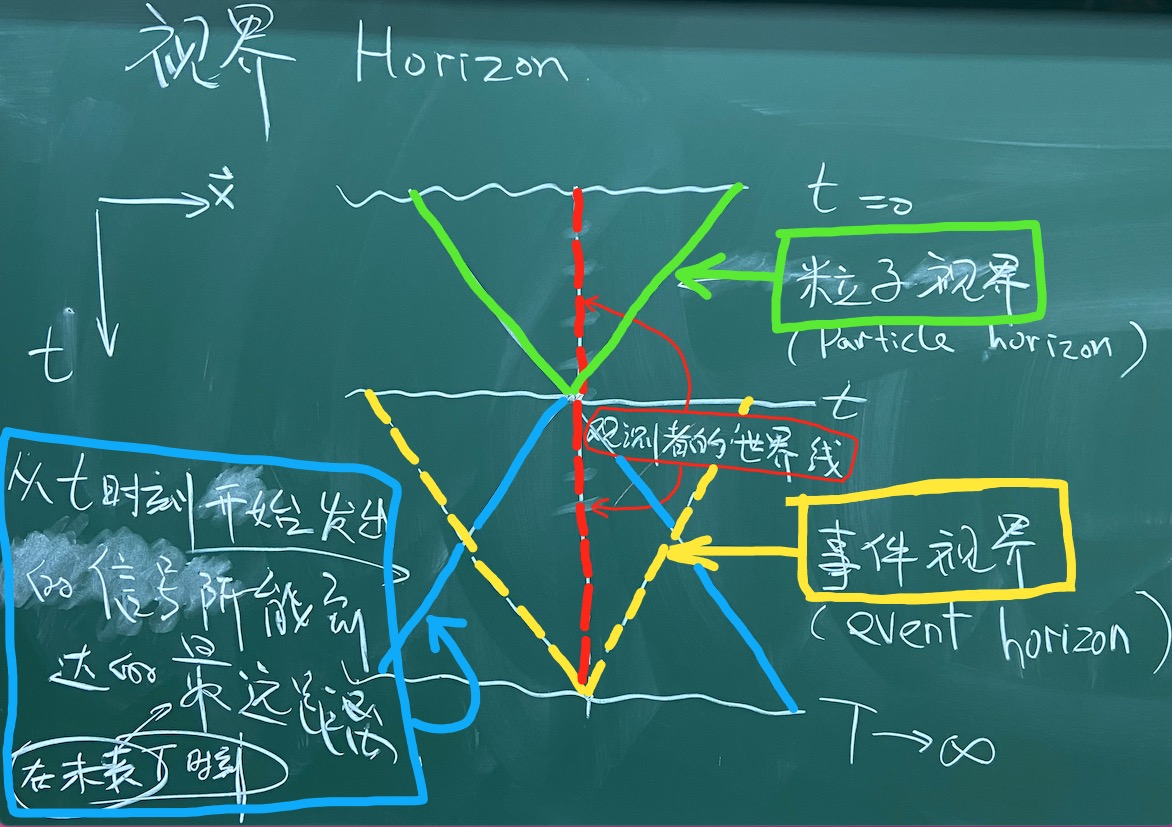
\includegraphics[width=1.0\linewidth]{horizon.jpg}
	\caption{视界}
\end{figure}


\section{宇宙学常数和真空能}

\subsection{真空能视角}
真空能 $P=-\rho$.

\begin{equation} 
    T^\mu_{\nu} = \left(\begin{array}{llll}-\rho & 0 & 0 & 0 \\ 0 & P & 0 & 0 \\ 0& 0& P &0 \\ 0 & 0&0&P\end{array}\right) = -\rho \delta^\mu_{\nu}
\end{equation}
得到真空能的能动量张量 $T_{\mu\nu}^{(\Lambda)}=- \rho_\Lambda g_{\mu\nu}$.

Einstein场方程 $R_{\mu\nu} - \frac{1}{2} g_{\mu\nu} R = -8\pi G T_{\mu\nu}$.
其中 $R_{\mu\nu}$ 是 Ricci tensor,  $R$ 是 Ricci scalar, 二者都是  $g_{\mu\nu}$ 及其导数的函数。

$T_{\mu\nu}$ 是能动量张量,包括物质和辐射(下式第一项)和真空能(下式第二项)

\begin{equation}
    T_{\mu\nu} = T_{\mu\nu}^{(M)} + T_{\mu\nu}^{(\Lambda)} = T_{\mu\nu}^{(M)} - \rho_\Lambda g_{\mu\nu}
\end{equation}

此时场方程变成 
\begin{equation} \label{Eeq.vacuum}
    R_{\mu\nu} - \frac{1}{2} g_{\mu\nu} R = -8\pi G T_{\mu\nu} =  -8\pi G T_{\mu\nu}^{(M)} +  8\pi G \rho_\Lambda g_{\mu\nu}
\end{equation}

\subsection{宇宙学常数视角}
Einstein场方程是由作用量导出的。作用量$S$为

\begin{equation}
    S = \int d^4 x \sqrt{-g} \mathcal{L} 
\end{equation}
其中 $d^4 x \sqrt{-g}$ 是4维协变的体积元,$\mathcal{L}$ 是拉氏量密度,要求 
\begin{itemize}
    \item[1.] 是4维坐标变换下的不变量。
    \item[2.] 包含度规的最高2阶导数。
\end{itemize}

只有Ricci scalar同时满足这两个条件,还有一个平凡(trivial)解——常数。 把宇宙学常数加到作用量里:
\begin{equation}
    S = \int d^4 x \sqrt{-g} \left( R  + \Lambda \right) 
\end{equation}
导出的场方程为
\begin{equation}
    R_{\mu\nu} - \frac{1}{2} g_{\mu\nu} R - \Lambda g_{\mu\nu} =  -8\pi G T_{\mu\nu}^{(M)} 
\end{equation}

与 \refeq{Eeq.vacuum} 相比,可得
\begin{equation}
    \Lambda = 8\pi G \rho_\Lambda 
\end{equation}

真空能与宇宙学常数是等价的。只不过真空能的引入有一些量子场论中的动机,而宇宙学常数则来自对广义相对论的Einstein场方程理论上的推广。下面我们将混用“真空能”和“宇宙学常数”。

\subsection{Einstein静态宇宙模型}

静态宇宙模型要求 $a$ 为常数,$\dot{a}=\ddot{a}=0$,带入弗里德曼方程得到
\begin{eqnarray}
    \rho+3P&=&0 \\
    K &=& \frac{8}{3} \pi G \rho a^2
\end{eqnarray}

如果只有物质和辐射,$\rho+3P>0$,所以Einstein在1917年引入了宇宙学常数。以下推导使用真空能,且忽略辐射。
\begin{equation}
    \begin{aligned}
    &\rho=\rho_{M}+\rho_{\Lambda}\\
    &P=P_{M}+P_{\Lambda}=-\rho_{\Lambda}\\
    &\rho+3 P = 0 \\
    & \Rightarrow \rho_{\Lambda}=\frac{1}{2} \rho_{M}
    \end{aligned}
\end{equation}

\begin{equation}
    K=\frac{8}{3} \pi G \rho a_{E}^{2}=8\pi G \rho_\Lambda a_{E}^{2}>0
\end{equation}

所以是正曲率,$K=+1$,

\begin{equation}
    a_E = 1/\sqrt{8\pi G \rho_\Lambda}
\end{equation}

但这个解不稳定。我们做微扰:
\begin{eqnarray}
    a&=&a_{E}+\delta a \\ 
    \rho_{M}&=&2 \rho_\Lambda+\delta \rho \\ 
\end{eqnarray}

要总满足
\begin{equation}
    1=\frac{8}{3} \pi G \rho a^{2}
\end{equation}

\begin{equation}
    \delta a<0 \Rightarrow \delta \rho>0 
\end{equation}
使得 $\dot{a}=0$ 继续满足,但二阶导

\begin{equation}
    \frac{3 \ddot{a}}{a}=-4 \pi G(\rho+3 P)=-4 \pi G\left(3 \rho_\Lambda+\delta \rho-3 \rho_\Lambda\right)=-4 \pi G \delta \rho<0
\end{equation}

$\delta a<0  \Rightarrow \ddot{a}<0$,
$\delta a>0  \Rightarrow \ddot{a}>0$,
即静态模型不稳定。


\section{早期宇宙的历史}

本章会讲3个重要的话题:
\begin{itemize}
    \item CMB 微波背景辐射
    \item BBN 大爆炸核合成
    \item Inflation 暴涨宇宙
\end{itemize}

\section{微波背景辐射}

\subsection{退耦(decoupling)}

自由质子和自由电子复合成中性氢原子,放出光子(大于等于13.6 eV),中性氢原子也可以吸收光子电离为自由的质子和电子。

随着宇宙膨胀,光子能量降低,复合率逐渐变得远大于电离率。
具体地说,当 $k_B T =0.3 \mathrm{~eV}$ 时,复合率远大于电离率。

另一方面,当光子和电子的散射速率小于宇宙膨胀速率后,光子和电子退耦。

光子被电子散射的速率 $\Lambda_\gamma = \sigma_T n_e v$,其中 $\sigma_T$ 是Thomson散射截面,$n_e$ 是电子数密度, $v$是电子运动速度。早期运动速度接近光速,$\Lambda_\gamma \simeq \sigma_T n_e c \propto a^{-3} \propto \left(T/T_{\gamma 0}\right)^3 $ 其中$T_{\gamma 0}$ 是今天CMB的温度。

宇宙膨胀速率,在辐射占主导期, $H\propto a^{-2} \propto \left(T/T_{\gamma 0}\right)^2$ 。早期散射速率远大于膨胀速率,能达到化学平衡。但散射速率降得更快,当散射速率小于宇宙膨胀速率,化学平衡被打破。

在化学平衡中的等离子体中,光子不断被散射,宇宙对光子是不透明的(opaque),化学平衡被打破时,光子不再发生散射,而是惯性运动,形成最后散射面。最后散射面由被我们观测到的CMB光子的最后一次散射位置组成,近似为一个二维球面。见\reffig{fig.LastScat}

\begin{figure}[!hbtp]
	\centering
	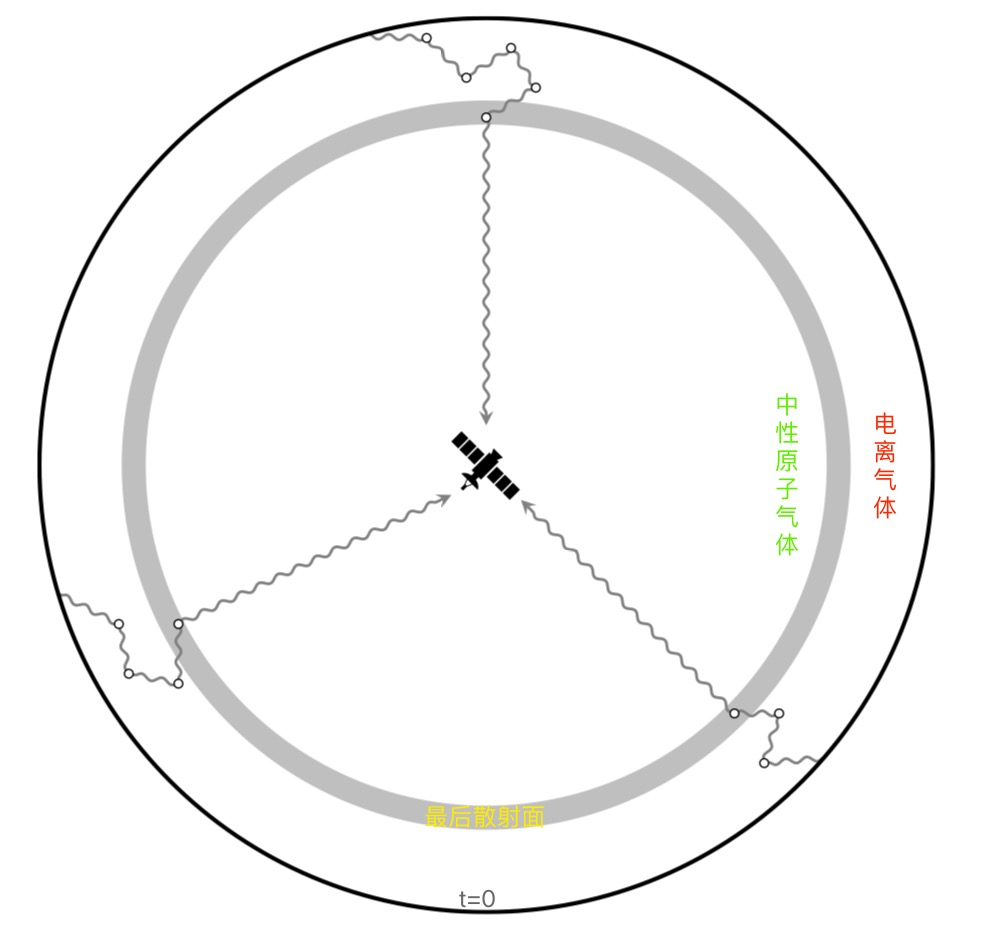
\includegraphics[width=1.0\linewidth]{lastScatter2022.jpg}
	\caption{图中灰色圆环为最后散射面,修改自 Daniel Baumann: Cosmology (2021)} \label{fig.LastScat}
\end{figure}

\subsection{CMB的特征}

\begin{itemize}
    \item 各向同性:来自所有方向的CMB温度高度相同。
    \item 辐射场强度随频率的分布符合黑体辐射谱。(Planck公式)
    \item 退耦能标约为 $0.3\mathrm{eV}$,温度约为3000K,红移约为1100
    \item 温度涨落有偶极矩。(因为地球、太阳、银河系的运动。)
    \item 扣除偶极矩后,仍然存在微小的温度起伏,这就是后来宇宙密度起伏、形成星系等结构的种子/初始条件。
\end{itemize}

为什么CMB符合黑体谱?

在最后散射面 $t_L$,光子辐射谱满足Planck公式:
\begin{equation}
    n_{T(t_L)}(\nu_L) d \nu_L=\frac{8 \pi \nu_L^{2} d \nu_L}{\exp \left(\frac{h_\text{pl} \nu_L}{k_{B} T(t_L)} \right)-1}
\end{equation}
在$t>t_L$,光子频率由于宇宙学红移降低 $\nu=\nu_{L} \frac{a(t_L)}{a(t)}$,
光子数密度 $n\left(\nu, t\right) d\nu \propto a^{-3}$即
\begin{equation}
    n(\nu, t) d \nu=\left(\frac{a(t_L)}{a(t)}\right)^{3} n_{T\left(t_{L}\right)}\left(\nu_{L}\right) d \nu_{L}
\end{equation}

代入得
\begin{equation}
    n(\nu, t) d \nu = \frac{8 \pi \nu^{2} d \nu}{\exp \left(\frac{h_\text{pl} \nu}{k_{B} \frac{a(t_L)}{a(t)}T(t_L)}   \right)-1}
\end{equation}
仍然是黑体谱。此时光子不处于热平衡,不妨令$T(t)=\frac{a(t_L)}{a(t)}T(t_L)$,即$T\propto 1/a$.

\section*{微波背景辐射(续)}

\subsection*{光子、核子密度}

光子的能量密度 $\rho_\gamma = \int h_{\mathrm{pl}} \nu n(\nu) d\nu = a_B T^4$, 其中 $a_B=\frac{8\pi^5 k_B^4}{15 h_{\mathrm{pl}}^3 c^3 } = 7.566\times 10^{-15} \mathrm{~erg~cm^{-3}K^{-4}}$.

今天 $T_{\gamma,0} = 2.725 \mathrm{K}$, $\rho_{\gamma,0}=a_B T_{\gamma,0}^4 = 4.64\times 10^{-34} \mathrm{~g~cm^{-3}}$ (erg和g之间用 $E=mc^2$ 换算),
$\Omega_\gamma = \frac{\rho_{\gamma,0}}{\rho_\text{crit}} = 2.47\times 10^{-5} h^{-2} \simeq 5\times 10^{-5}$.

今天的总辐射包括光子和中微子。中微子作为费米子,和光子的统计不同。且中微子退耦更早,所以温度低于光子。最后,中微子有3种。总结如下
\begin{equation}
    \rho_{R, 0}=\rho_{\gamma, 0}+\rho_{\gamma, 0} \times\left(\frac{7}{8}\right) \times\left(\frac{4}{11}\right)^{4 / 3} \times 3 =7.80 \times 10^{-34} \mathrm{~g~cm^{-3}}
\end{equation}

总之今天辐射的能量密度远远小于冷物质和暗能量。
\begin{equation}
    \begin{aligned}
        \Omega_{R}=\frac{\rho_{R, 0}}{\rho_\text{crit}} &=4.15 \times 10^{-5} h^{-2} \\
        & \simeq 8.3 \times 10^{-5} \ll \Omega_M, \Omega_\Lambda
    \end{aligned}
\end{equation}

考虑光子的数密度
\begin{equation}
    n_{\gamma}=\int_{0}^{\infty} n_{T}(\nu) d \nu=\frac{30 \zeta(3)}{\pi^{4}} \frac{a_{B}}{k_{B}} T^{3}=20.28 T^{3} \mathrm{~cm}^{-3}
\end{equation}

今天 $T_{\gamma,0} = 2.725 \mathrm{K}$, $n_{\gamma, 0}=410$ photons $/ \mathrm{cm}^{3}$

核子数密度
\begin{equation}
    n_{B, 0}=\frac{\rho_{B, 0}}{m_{N}}=\frac{\Omega_{B} \rho_{\text {crit }}}{m_{N}}=1.123 \times 10^{-5} \Omega_{B} h^{2} \text { nucleons } / \mathrm{cm}^{3}
\end{equation}
其中 $m_{N}$ 是核子平均质量。

光子与核子数密度比
% $$
% \frac{n_{\gamma}}{n_{B}}=\frac{n_{\gamma,0}}{n_{B, 0}}=3.65 \times 11^{7} /\left(\Omega_{B} h^{2}\right) \simeq 2.4\times 10^9
% $$
\begin{equation}
    \eta = \frac{n_{B}}{n_{\gamma}} \simeq 4.1\times 10^{-10}
\end{equation}

上节课讲过,在绝热膨胀的宇宙中,为了保持普朗克黑体辐射谱,我们定义非热平衡的光子的温度正比于$a$的$-1$次方。
对于非相对论性粒子,为了遵循玻尔兹曼统计,温度正比于$a$的$-2$次方。
在退耦前,光子和核子处于热平衡,光子远多于核子,占据主导,温度正比于$a$的$-1$次方。

\subsection*{估算光子退耦时刻}

散射速率
\begin{equation}
    \Lambda_\gamma=\sigma_{T} n_{e} c=0.88 n_{B,0}\left(\frac{T}{T_{\gamma,0}}\right)^{3} \sigma_{T} c=1.97 \times 10^{-19} \mathrm{~s}^{-1} \Omega_{\mathrm{B}}{h }^{2}\left(T / T_{\gamma,0}\right)^{3}
\end{equation}

其中用到平均一个核子对应$Y_H+\frac{1}{2}Y_{He}=0.76+\frac{1}{2}\times 0.24=0.88$个电子。

能量转移速率
\begin{equation}
    \Gamma \gamma \simeq\left(\frac{\Delta E}{k_{B} T}\right) \Lambda_{\gamma} \approx\left(\frac{k_{B} T}{m_{e} c^{2}}\right) \Lambda_{\gamma} \simeq 9.0 \times 10^{-29} s^{-1} \Omega_{B} h^{2}\left(\frac{T}{T_{\gamma,{0}}}\right)^{4}
\end{equation}

而宇宙膨胀速率(假设辐射占主导)
\begin{equation}
    \begin{aligned}
        H=\frac{\dot{a}}{a} & \approx H_{0} \sqrt{\Omega_R\left(T / T_{\gamma,{0}}\right)^{4}} \\
    &=2.1\times 10^{-20} s^{-1} \left(\frac{T}{T_{\gamma,{0}}}\right)^{2}
    \end{aligned}
\end{equation}

能量转移速率比膨胀速率下降快,当 $\Gamma_{\gamma} \leq H$ ,散射速率不足,光子与重子物质退耦,也可以叫freeze out.此时温度约为$10^5 \mathrm{~K}$.
但后面会看到,这样估算出的温度过高,处于辐射为主的阶段,是不准确的。

\subsection*{物质-辐射相等时刻}
辐射的能量密度正比于$a$的$-4$次方,冷物质的能量密度正比于$a$的$-3$次方,辐射密度下降快,辐射在宇宙早期先占据主导,后来下降到小于冷物质的能量密度,二者相等的时刻叫做“物质-辐射相等时刻”(matter-radiation equality epoch).
\begin{equation}
    T_{eq}=T_{\gamma,0}\left(\frac{\Omega_{M}}{\Omega_{R}}\right)=6.56 \times 10^{4} \Omega_{m} h^{2} \mathrm{~K} =10^{4} \mathrm{~K}
\end{equation}
一般使用红移表示
\begin{equation}
    1+z_{eq}=\left(\frac{a_{e q}}{a_{0}}\right)^{-1}=\frac{\Omega_{M}}{\Omega_{R}}=2.4 \times 10^{4}\left(\Omega_M h^{2}\right) \simeq 3500
\end{equation}

\subsection*{Boltzmann方程和Saha方程}
对于反应 $1+2 \longleftrightarrow 3+4$,
非平衡态下的Boltzmann方程为
\begin{equation}
    a^{-3} \frac{d}{d t}\left(n_{1} a^{3}\right)=n_{1}^{(0)} n_{2}^{(0)}\langle\sigma v\rangle\left(\frac{n_{3} n_{4}}{n_{3}^{(0)} n_{4}^{(0)}}-\frac{n_{1} n_{2}}{n_{1}^{(0)} n_{2}^{(0)}}\right)
\end{equation}
其中 $\langle\sigma v\rangle$ 是 thermally averaged cross-section. 括号中第一项度量了反应向左移动的速率,第二项度量了反应向右移动的速率。
\begin{equation}
    n_{i}^{(0)}=\left\{\begin{array}{l}
    g_{i}\left(\frac{m_i T}{2 \pi}\right)^{3 / 2} e^{-\frac{m_{i} c^{2}}{k_{B} T}  }, \qquad m_{i} c^{2}\gg k_{B} T \\
    \frac{g_{i}^{3}}{\pi^{2}}T^3, \qquad m_{i} c^{2}\ll k_{B} T 
    \end{array}\right.
\end{equation}

平衡态下的精细平衡方程
\begin{equation}
    \frac{n_{3} n_{4}}{n_{3}^{(0)} n_{4}^{(0)}}=\frac{n_{1} n_{2}}{n_{1}^{(0)} n_{2}^{(0)}}
\end{equation}

具体到再复合(recombination),反应是 $e+p \leftrightarrow H+\gamma$.
代入精细平衡方程得到Saha方程
\begin{equation}
    \frac{n_{e}n_p}{n_{H}}=\frac{n_{e}^{(0)} n_{p}^{(0)}}{n_{H}^{(0)}}
\end{equation}

其中光子的化学势为0,$n_\gamma = n_{\gamma}^{(0)}$.
忽略He贡献,电子数密度与质子数密度近似相等
$$n_{e}=n_{p}=X_{e} n_{b}$$
其中$n_{b}=n_{p}+n_{H}$ 是重子数密度,$X_e$ 是电离度。剩下的H以中性原子形式存在
$$n_{H}=\left(1 - X_{e}\right) n_{b}$$

此时温度远小于质子和电子的能标,使用非相对论情形计算$n_i^{(0)}$
\begin{eqnarray}
      \frac{n_{e}^{(0)} n_{p}^{(0)}}{n_{H}^{(0)}} &=& \frac{g_e g_p}{g_H} \left(\frac{m_e m_p}{m_H}\right)^\frac{3}{2} \left(\frac{T}{2\pi }\right)^\frac{3 }{2} e^{-\frac{B_1}{k_B T}} \\ 
      &\simeq&\left(\frac{m_e T}{2\pi }\right)^\frac{3 }{2} e^{-\frac{B_1}{k_B T}}
\end{eqnarray}

  
其中 $B_1=m_e+m_p - m_H=13.6\mathrm{eV}$ 是中性氢原子的结合能, 自由度 $g_e=2,g_p=2,g_H=4$.

Boltzmann方程左边
\begin{equation}
    a^{-3} \frac{d}{d t}\left(n_{e} a^{3}\right)= a^{-3} \frac{d}{d t}\left(X_{e} n_{b} a^{3}\right) = n_b \frac{d X_e}{dt}
\end{equation}

即
\begin{eqnarray}
    n_b \frac{d X_e}{dt} &=& n_{e}^{(0)} n_{p}^{(0)}\langle\sigma v\rangle\left(\frac{n_H}{n_{H}^{(0)}}-\frac{n_{e} n_{p}}{n_{e}^{(0)} n_{p}^{(0)}}\right)   \\ 
    &=& (1-X_e) n_b \langle\sigma v\rangle \frac{n_{e}^{(0)} n_{p}^{(0)}}{n_H^{(0)}} - X_e^2 n_b^2 \langle\sigma v\rangle \\
    &=& (1-X_e) n_b \beta  - X_e^2 n_b^2 \alpha^{(2)}
\end{eqnarray}
其中
\begin{equation}
    \beta \equiv \langle\sigma v\rangle\left(\frac{m_{e} T}{2 \pi}\right)^\frac{3 }{2} e^{-\frac{B_1}{k_B T}}
\end{equation}
\begin{equation}
    \alpha^{(2)} \equiv \langle\sigma v\rangle=9.78 \frac{\alpha^{2}}{m_{e}^{2}}\left(\frac{B_{1}}{k_{B} T}\right)^\frac{1 }{2} \ln \left(\frac{B_{1}}{k_{B} T}\right)
\end{equation}

得到Boltzmann方程
\begin{equation}
    \frac{d X_{e}}{d t}=\left(1-X_{e}\right) \beta-X_{e}^{2} n_{b} \alpha^{(2)}
\end{equation}

再复合开始时,$\frac{d X_{e}}{d t}=0$, $\text{RHS}=0$,即Saha方程
\begin{equation}
    \frac{X_{e}^{2}}{\left(1-X_{e}\right)} = \frac{\beta}{n_{b} \alpha^{(2)}} = \frac{1 }{n_b} \left(\frac{m_{e} T}{2 \pi}\right)^\frac{3 }{2} e^{-\frac{B_1}{k_B T}}
\end{equation}
指数项占主导。

解Saha方程的结果是退耦发生在$z\sim 1100$, $T\sim 3000\mathrm{K}$时。

但是Saha方程的解是电离度一直随exp指数下降,这是不准确的。考虑到退耦后平衡态被打破,应使用非平衡态的Boltzmann方程求解,则可以正确地给出退耦后的残余电离度约为$10^{-3}$,见下图(引自Dodelson)。
\begin{figure}[!hbtp]
	\centering
	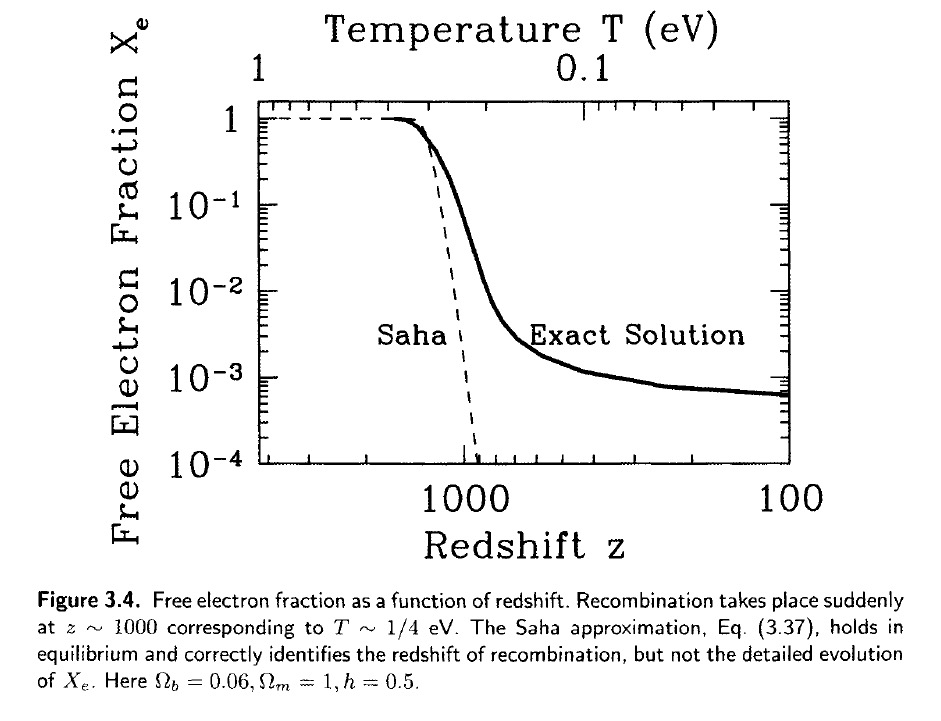
\includegraphics[width=1.0\linewidth]{recombination.jpg}
	\caption{再复合时期电离度的下降} 
\end{figure}


\section{CMB的偶极各向异性(dipole anisotropy)}

光子数密度符合普朗克公式
\begin{equation}
    n_T\left(\nu\right) d\nu = \frac{8\pi \nu^2 /c^3}{e^\frac{h\nu}{k_BT}-1} d\nu
\end{equation}

我们求相空间的数密度。相空间(坐标和动量组成的参数空间)的粒子数量 $N\left(\boldsymbol{x},\boldsymbol{p}\right) d^3x d^3p$是守恒量, 其中$d^3x d^3p$是相空间的体积元,是 Lorentz 不变量, 因此$N\left(\boldsymbol{x},\boldsymbol{p}\right)$也是Lorentz不变量。

对于光子, $|\boldsymbol{p}|=E/c=h_{\mathrm{pl}} \nu/c$,则 $d^3p=4\pi |\boldsymbol{p}|^2 dp=4\pi h_{\mathrm{pl}}^3 \nu^2/c^3 d\nu$. 且对于光子, $N_\gamma(\boldsymbol{x},\boldsymbol{p})=N_\gamma\left(p\right) $

光子数一定,
\begin{equation}
    N_\gamma(p)d^3x d^3p = \frac{1}{2} n_T\left(\nu\right) d\nu d^3x
\end{equation}
其中1/2是因为光子有两种极化。

得到 
\begin{equation}
    N_\gamma(p) = \frac{1}{h_{\mathrm{pl}}^3} \frac{1}{e^\frac{pc}{k_B T}-1}
\end{equation}

地球(以下带$'$的是地球坐标系)相对 共动坐标系有一个相对运动速度
$v = \mathcal{O} \left(100 \mathrm{km/s}\right) $, 
此时相对论的速度参数
$\beta \equiv v/c\sim 10^{-3}$,
$\gamma \equiv \left(1-\beta^2\right)^{-\frac{1}{2}}\sim 1$. 
设地球上观测到的光子动量$\boldsymbol{p'}$与地球坐标系运动速度$\boldsymbol{v}$夹角是$\theta$,$|\boldsymbol{p}| =\gamma \left(1+\beta \cos \theta \right) |\boldsymbol{p^\prime}|$
则
\begin{equation}
    N_\gamma^\prime(p') = \frac{1}{h_{\mathrm{pl}}^3} \frac{1}{e^\frac{p'c}{k_B T'}-1}
\end{equation}
\begin{equation}
    T'\left(\theta\right) = \frac{T}{\gamma \left(1+\beta \cos \theta\right) } \simeq T\left(1-\beta \cos \theta\right) 
\end{equation}
可以观测到偶极各向异性,其中$\theta=0$时(光子从后方追上观察者),观测到的温度$T'$偏低,$\theta=\pi$时(光子迎面而来),观测到的温度$T'$偏高。

实际观测到的CMB偶极矩说明了地球相对于“CMB frame”有运动。
扣除这个偶极矩后,我们可以得到宇宙真实的密度起伏。


\section{大爆炸核合成 \\(Big Bang Nucleosynthesis, BBN)}

对于一种原子核,原子序数 $Z$,
原子质量数 $A$, 原子核质量$m$, 中子质量 $m_n$, 质子质量$m_p$.
束缚能
\begin{equation}
    B=Z m_p + (A-Z) m_n -m
\end{equation}
质子中子能量差 $Q=m_n-m_p = 1.293 \mathrm{~MeV}$,
氘核结合能 $B_D = 2.22 \mathrm{~MeV} $.
% 比结合能约为 $1.11 \mathrm{~MeV} $, 小于质子中子能量差,所以 

大爆炸核合成的预言:
\begin{itemize}
    \item[1.] 轻元素(H, He, 部分 Li, C)在大爆炸中合成。
    \item[2.] 定量预言 H, He, Li, C 的丰度。
\end{itemize}

质子和中子通过弱相互作用可以相互转化。
\begin{eqnarray}
    p+\bar{\nu} \leftrightarrow n + e^+ \\ 
    p + e^- \leftrightarrow n + \nu \\ 
    n \leftrightarrow p + e^- + \bar{\nu}
\end{eqnarray}

% 第一步,“形成”更多的中子。
当温度降低到 $T\sim 0.1 \mathrm{~MeV}$ 时,反应向产生中子的一端移动, 质子转化成中子。
中子足够多后(当$T\sim 0.07 \mathrm{~MeV}$)就可以形成轻元素。
\begin{eqnarray}
    p+n \leftrightarrow D + \gamma \\ 
    D + D \leftrightarrow \ce{^{3}He} + n \\ 
    \ce{^{3}He} + D \leftrightarrow \ce{^{4}He} + p  
\end{eqnarray}

% 中微子 abundance 【【??】】

考虑 $T > 0.5 \mathrm{~MeV}$,% 光子、中微子、正负电子均为相对论性
平衡态方程
\begin{equation}
    \frac{n_p}{n_n} = \frac{n_p^{(0)}}{n_n^{(0)}} = e^\frac{Q}{k_B T}
\end{equation}

定义
$X_n\equiv \frac{n_n}{n_b} = \frac{n_n}{n_n+n_p}$,
即
\begin{equation}
    \frac{1-X_n}{X_n} = \frac{n_p}{n_n} = e^\frac{Q}{k_B T}
\end{equation}

(提问补充:在中微子退耦前,反应向质子一方移动。)

反应发生后需要使用非平衡态的Boltzmann方程,
\begin{equation}
    \frac{dX_n}{dt} = \lambda_{np} \left( \left(1-X_n\right) e^{-\frac{Q }{k_B T}}-X_n\right) 
\end{equation}

其中速率 $\lambda_{np} = \frac{255}{\tau_n x^5} \left(12+6x+x^2\right) $,  
$x=\frac{Q}{k_B T}$.
当$T\simeq 0.5 \mathrm{~MeV}$时,
$X_n \simeq 0.15$,
中子寿命$\tau_n \simeq 15\mathrm{min} \simeq 886.7 \mathrm{sec}$.

轻元素形成时,温度$T_\text{nuc}\sim 0.07 \mathrm{~MeV}$, 
\begin{equation}
    X_n\left(T_\text{nuc}\right) = 0.15 \exp\left(-\frac{t }{\tau_n}\right) =0.11
\end{equation}

BBN时期的宇宙辐射占主导,$t\propto a^2\propto T^{-2}$. 所以此时宇宙的年龄为
\begin{equation}
    t = 132 \mathrm{sec} \left(\frac{0.1 \mathrm{~MeV}}{T}\right)^2 =   132 \mathrm{sec} \left(\frac{0.1 }{0.07}\right)^2 \simeq 269 \mathrm{sec}
\end{equation}

\begin{figure}[!hbtp]
	\centering
	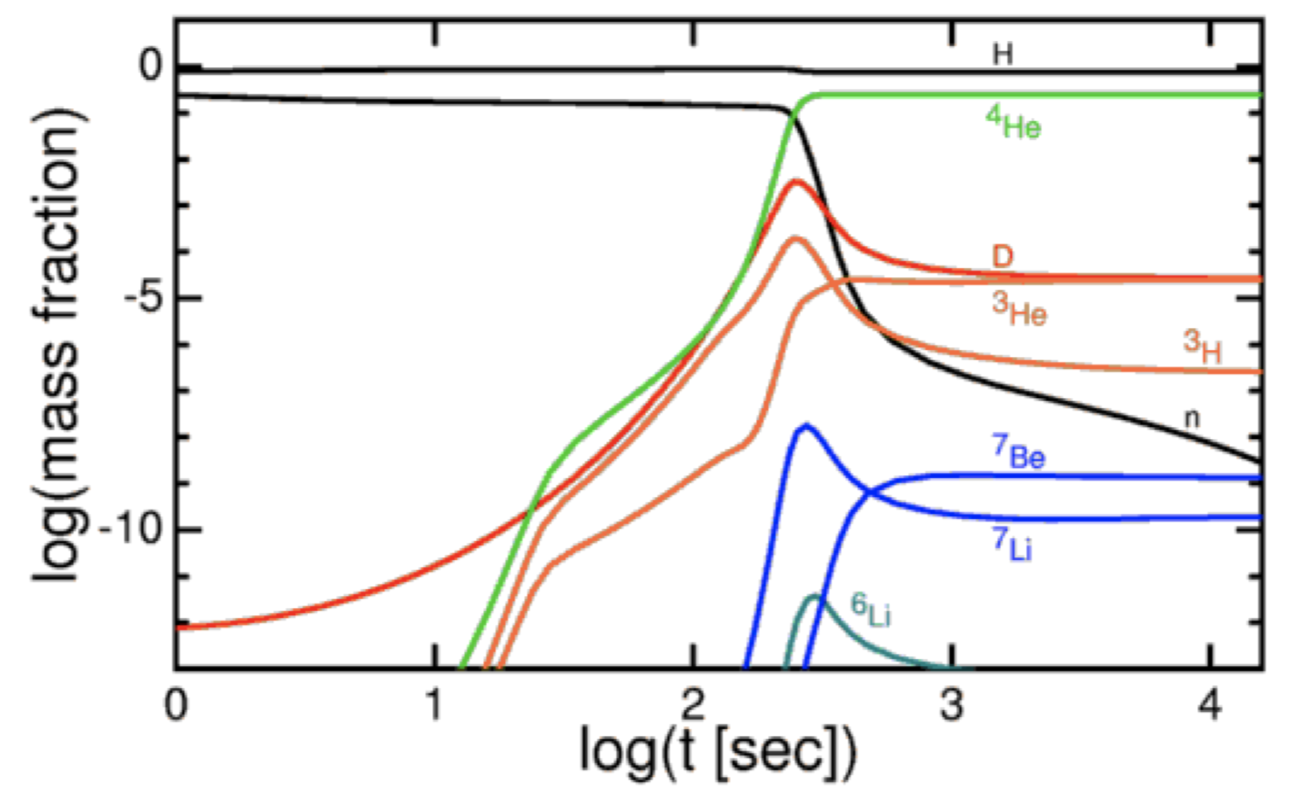
\includegraphics[width=1.0\linewidth]{BBNt.png}
	\caption{轻元素丰度随时间的变化(图源Hannu Kurki-Suonio)} \label{fig:BBNt}
\end{figure}

BBN期间各种原子核质量占比随时间的演化如 \reffig{fig:BBNt}   所示,可以看到BBN结束时,
多数中子都进入了$\ce{^{4}He} $, $X_{\ce{^{4}He} } \equiv \frac{4 n_{\ce{^{4}He} }}{n_b} = 2X_n\left(T_\text{nuc}\right) =0.22$.
这是估算,精确的结果是
\begin{equation}
    X_{\ce{^{4}He} } = 0.2262+0.0135 \ln \left( \frac{\eta_b}{10^{-10}}\right) \approx 0.24
\end{equation}
其中$\eta_b = \frac{n_b}{n_\gamma} \simeq 4\times 10^{-10}$, 与 $\Omega_b h^2$有关。

如果忽略掉质子和中子质量微小的差异,
那么$X_{\ce{^{4}He}}$的物理意义就是氦4的质量丰度,
有时候用$Y_p$表示,即氦4核在所有核子里的质量比。
此外,也经常定义以数量计算的氦4丰度 $y_{\ce{^{4}He}}$,即氦4核在所有原子核里的数量比。
由于氢(H)原子核只包含1个核子,而氦4($\ce{^{4}He}$)原子核包含4个核子,所以\\
\begin{equation}
    y_{\ce{^{4}He}} = \frac{ \frac{1}{4} X_{\ce{^{4}He}}}{ (1- X_{\ce{^{4}He}}) +  \frac{1}{4} X_{\ce{^{4}He}} } \approx 0.0724
\end{equation}

\begin{figure}[!hbtp]
	\centering
	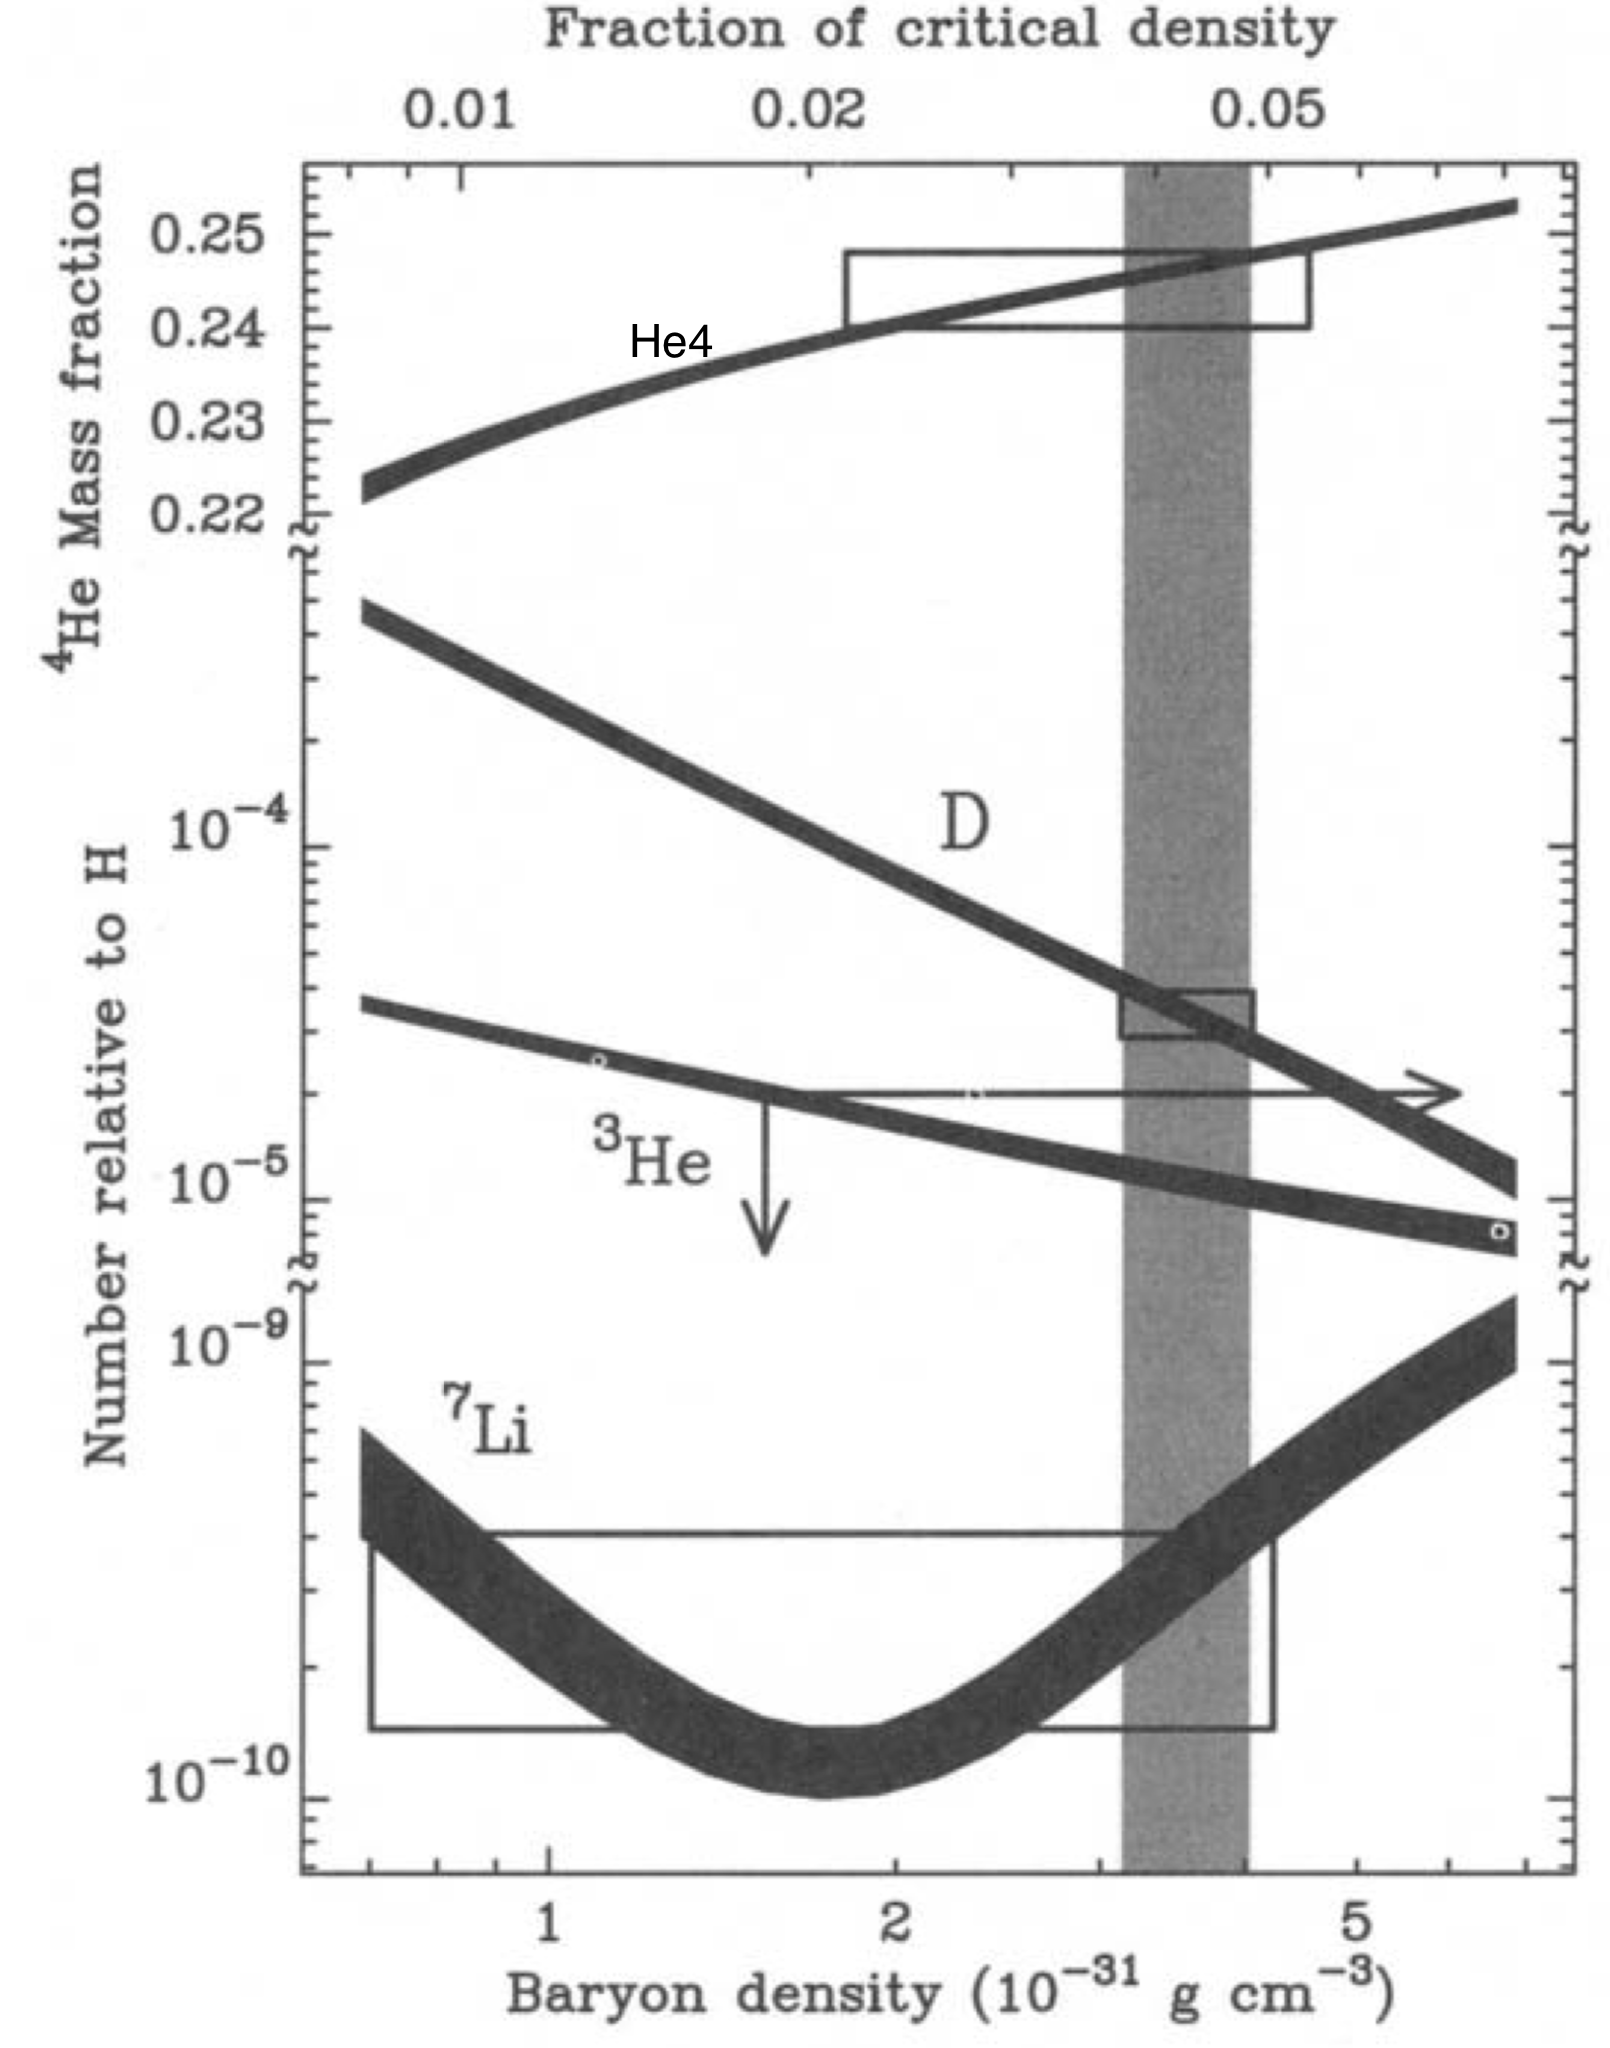
\includegraphics[width=1.0\linewidth]{BBN.png}
	\caption{轻元素丰度的预言和测量(图源Dodelson)} \label{fig:BBN}
\end{figure}

对BBN的测量见 \reffig{fig:BBN}。
从4个独立丰度测量得到自洽的 $\Omega_b h^2$ 限制。
\begin{eqnarray}
    \Omega_b \simeq 0.05 \\ 
    h\simeq 0.7 \\ 
    \Omega_b h^2 \simeq 0.025
\end{eqnarray}


\section{中微子退耦(neutrino decoupling)}

中微子退耦发生在约 $1 \mathrm{~MeV}$ 时。

在$T> 10 \mathrm{~MeV}$时,正负电子和正负中微子通过弱相互作用 $e^+ + e^- \leftrightarrow \nu + \bar{\nu}$ 互相转化达到热平衡,康普顿散射使电子和光子达到热平衡。此时质子、中子、电子、光子、中微子都处于热平衡之中。

当 $T \sim 1 \mathrm{~MeV}$ 时,弱相互作用的反应不够有效,中微子退耦。此时质子、中子、电子、光子处于热平衡之中。

当 $T \sim 0.5 \mathrm{~MeV}$ 时,即约为电子的静质量时,电子变成非相对论性粒子(注:正负电子湮灭),将部分能量转移给光子,导致光子温度上升。而此时中微子已经退耦,自行绝热膨胀,不会接收这部分能量,导致光子温度大于中微子。质子和中子比电子重很多,此时为非相对论粒子,虽然也处在热平衡中,但能量贡献不变,以下计算能量转移不考虑质子和中子。

以下计算光子(微波背景辐射)温度比中微子(背景辐射)温度高多少。

定义熵密度 $s(T) = \frac{\rho+P}{T}$,热平衡系统$s\propto a^{-3}$.
粒子数密度为(假设化学势为0)
\begin{equation}
    n(p) dp = \frac{4\pi g p^2}{h_{\mathrm{pl}}^3} \frac{1}{\exp\left(\frac{\sqrt{p^2+m^2}}{k_B T}\right) \pm 1}
\end{equation}
费米子(Fermion, 如电子、中微子)取正号,玻色子(Boson, 如光子)取负号。

能量密度
\begin{equation}
    \rho (T) = \int_0^\infty n(p,T) dp \sqrt{p^2+m^2}
\end{equation}

相对论性粒子
\begin{equation}
    \rho(T) =
    \begin{cases}
        \frac{1}{2} g a_B T^4   & \text{Boson} \\ 
        \frac{7}{8} \times \frac{1}{2} g a_B T^4 & \text{Fermion}
    \end{cases}
\end{equation}
其中$g$是粒子的简并度,包括粒子种类(比如中微子有三代)、正反粒子、自旋态。$a_B$是常数。
记为 $\rho(T) = \frac{1}{2} \mathcal{N} a_B T^4 $, 则
\begin{equation}
    \mathcal{N} =
    \begin{cases}
        g  & \text{Boson} \\ 
        \frac{7}{8} \times g  & \text{Fermion}
    \end{cases}
\end{equation}

对相对论性粒子,$P=\frac{1}{3}\rho$.
代入熵密度定义得到
$s(T) = \frac{4\rho}{3T} = \frac{2}{3} \mathcal{N} a_B T^3$,
由于$s(T) a^3 = const.$,
所以 
$\mathcal{N} a^3 T^3 = const.$

中微子退耦时间$t_\text{dec}$,此时温度 $T_\nu(t_\text{dec}) = T_\gamma(t_\text{dec}) = T_\text{dec}$.

\begin{equation}
    \mathcal{N}_\text{dec} = 2+ 1\times 2\times 2\times \frac{7}{8} = \frac{11}{2}
\end{equation}
其中第一项来自光子,第二项来自电子,其中1、2、2分别对应电子的种类、正反粒子、两个自旋态。

当 $t_* \gg t_\text{dec}$, 电子变成非相对论性粒子,不再考虑,所以
\begin{equation}
    \mathcal{N}(t_*) = 2
\end{equation}

中微子退耦后,自行按照 $T_\nu \propto \frac{1}{a}$ 演化,不受 $\mathcal{N}$ 变化的影响,所以
$T_\text{dec} a_\text{dec} = T_\nu (t_\text{dec}) a_\text{dec} = T_\nu(t_*) a(t_*)$.
由于光子和电子共同处于热平衡,所以 
\begin{equation}
    \mathcal{N}_\text{dec} a_\text{dec}^3 T_\text{dec}^3 = \mathcal{N}(t_*) a^3(t_*) T_\gamma^3(t_*)
\end{equation}
可以得到
\begin{equation}
    \frac{T_\nu(t_*)}{T_\gamma(t_*)} = \left(\frac{\mathcal{N}(t_*)}{\mathcal{N}_\text{dec}}\right)^\frac{1}{3} = \left(\frac{4}{11}\right)^\frac{1}{3} \simeq \frac{1}{1.4} 
\end{equation}

此后,光子和中微子都按照 $T\propto \frac{1}{a}$ 各自演化,可得今天
\begin{equation}
    \frac{T_{\nu,0}}{T_{\gamma,0}} = \frac{T_\nu(t_*)}{T_\gamma(t_*)} = \frac{1}{1.4}
\end{equation}

上面说的光子到今天红移到微波波段,即CMB。我们测量得到CMB的温度 $T_{\gamma,0}\simeq 2.725 \mathrm{~K}$, 则可推知中微子背景辐射 C$\nu$B 的温度$T_{\nu,0} \simeq 1.945 \mathrm{~K}$.

宇宙辐射能量密度
\begin{equation}
    \rho_{R,0} = \rho_{\gamma,0} + \rho_{\nu,0} = \frac{1}{2} a_B T_{\gamma,0}^4 \left(2+ 3\times 2\times 1\times\frac{7}{8} \times \left(\frac{4}{11}\right)^\frac{4}{3} \right) = 1.681 \rho_{\gamma,0}
\end{equation}
其中括号内第一项是光子,第二项是中微子,其中3、2、1分别对应中微子有三代(电子中微子$\nu_e$、缪子中微子$\nu_\mu$、陶子中微子$\nu_\tau$)、正反中微子、正反中微子各对应一个自旋态,7/8是由于中微子是费米子,$\left(\frac{4}{11}\right)^\frac{1}{3}$是中微子和光子的温度比,另外它的四次方因为能量密度正比于温度的4次方。

\section{暴涨理论(Inflation Theory)}

大爆炸理论中存在三个重要的疑难。

\subsection{平坦性问题(Flatness Problem)}
考虑物质主导的非平坦宇宙,
\begin{equation}
    \rho_m(t) = \Omega_M \rho_\text{crit} \left( \frac{a}{a_0}\right)^{-3}
\end{equation}

\begin{equation}
    |\Omega(t)-1| = \left|1+\frac{\Omega_M a_0}{\Omega_K a}\right|^{-1}
\end{equation}
%

假设 $\Omega_M = 0.9$, $\Omega_K = 0.1$, 
在 CMB 时期,$z=1000,  |\Omega(t)-1|  \simeq 10^{-4}$,
在 BBN 时期,$ |\Omega(t)-1|  \simeq  10^{-12}$.

可见即使今天的 $\Omega_K$ 不是很小,在宇宙早期  $\Omega_K$ 也是非常小的,这是需要解释的。

\subsection{视界疑难(Horizon Problem)}

CMB在全天$4\pi$立体角都高度各向同性,而CMB时期的粒子视界是有限大的。(注:除以角直径距离得到弧度)
\begin{equation}
    d_H (t_\text{CMB}) \simeq \frac{cH_0^{-1}}{\Omega_M^\frac{1}{2}\left(1+z_\text{CMB}\right)^\frac{3}{2} } \simeq 0.015 \mathrm{~rad} \sqrt{\Omega_M} \simeq 1^\circ 
\end{equation}
对应今天天空中的$1^\circ $, 天空中间隔超过$1^\circ $的两点在CMB时期并没有因果联系,它们的温度接近并不自然。

\subsection{磁单极子问题(Magnetic monopole)}

大统一理论(GUT)预言了磁单极子的存在,并且预言了较高的磁单极子密度。但是人们并没有观测到磁单极子。这个问题正是Alan Guth等人提出暴涨理论的动机。

\subsection{种子涨落的起源}

CMB的微小各向异性很难用热涨落解释,需要其它的起源。

\subsection{暴涨理论}

1981年,Alan Guth等人提出了暴涨理论。
暴涨理论认为宇宙极早期出现过一段指数膨胀的时期,$a\propto e^{Ht}$,在很短的时间内,宇宙膨胀了$e^{60}$倍,同时有某种物理机制使得暴涨结束。

\begin{itemize}
    \item 平坦性问题:暴涨前的宇宙可能有曲率,但暴涨使得我们今天的宇宙来自其中的一小块,所以很平坦。
    \item 视界疑难:暴涨后到CMB之间,辐射占主导,视界(注:在共动坐标系中)逐渐增大,但在暴涨时期,视界曾经随时间变小。原本有因果联系的两点退出彼此的视界,成为CMB上“没有因果联系”的两点,因此在暴涨后它们的温度仍然高度相同,如同处于热平衡。
    \item 磁单极子问题:暴涨使得磁单极子彼此急剧远离,导致今天的视界内平均不到一个磁单极子。
    \item 种子涨落的起源:暴涨使得微观上的量子涨落在短时间内被拉到宇宙的尺度上,成为经典的密度涨落。
\end{itemize}

\subsubsection*{如何实现暴涨?}

Alan Guth等人在1981年提出的简单模型:暴涨子在假真空态上提供相当于暗能量的效应,使宇宙加速膨胀,当暴涨子发生量子隧穿到达真的真空态上,暴涨结束。但是这样得出的种子涨落太大。如 \reffig{suichuan} 。

1982-1983年,Andrei Linde 改进提出慢滚模型(slow-roll),该模型中暴涨子在一个较平的假真空上缓慢滚动,当滚到真的真空态上时结束暴涨。如  \reffig{slow-roll} 。

慢滚模型是目前人们较为普遍接受的一种最简单的模型,但慢滚模型预言的原初引力波目前还没有观测到,因此有很多其它的暴涨模型,有待未来的观测告诉我们更多的信息。

\begin{figure}[!hbtp]
	\centering
	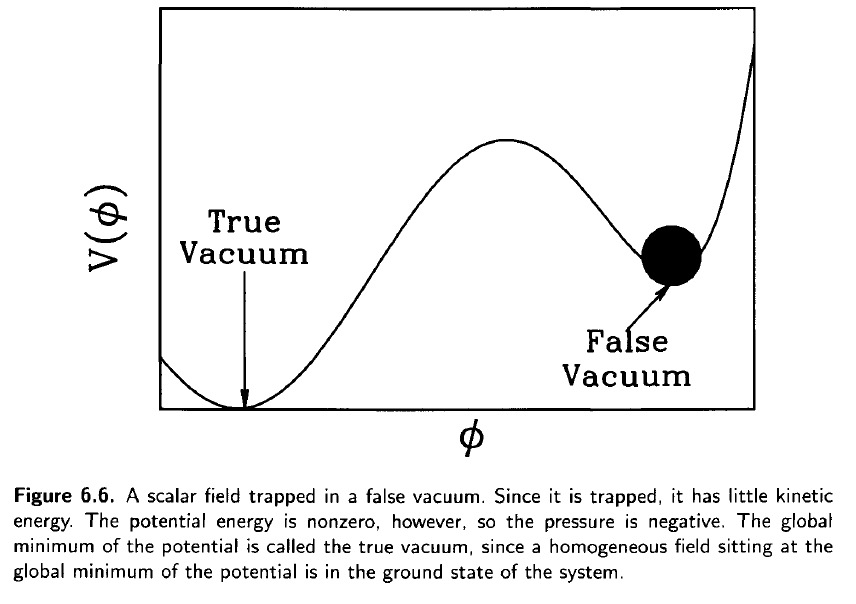
\includegraphics[width=1.0\linewidth]{suichuan.jpg}
	\caption{引自S. Dodelson.} \label{suichuan}
\end{figure}

\begin{figure}[!hbtp]
	\centering
	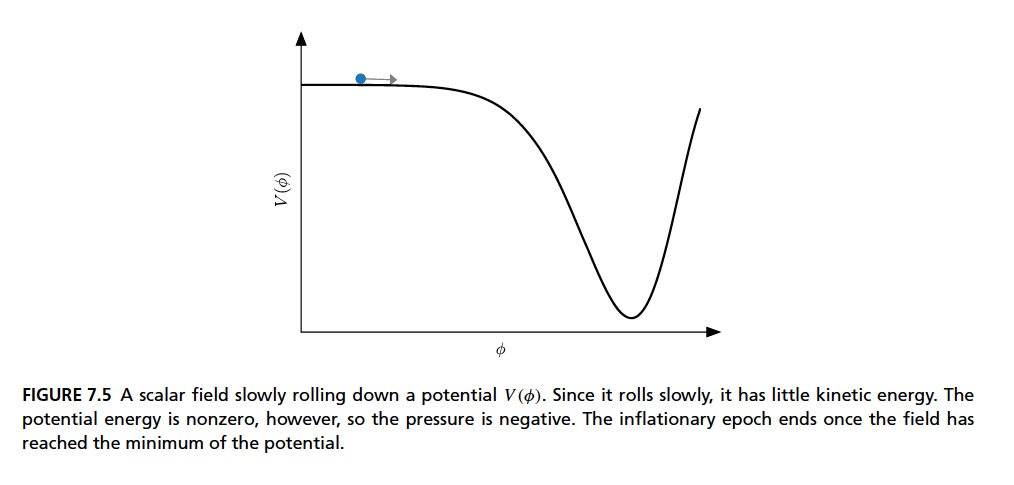
\includegraphics[width=1.0\linewidth]{slow-roll.jpg}
	\caption{引自 S. Dodelson \& F. Schmidt (second edition)} \label{slow-roll}
\end{figure}



\end{document}
